
% !TeX spellcheck = pt_BR
% !TEX encoding = UTF-8 Unicode

\chapter{Limites}\label{Cap:Limites}

\ifdefined\updateans
% Only need to run once in a lifetime, when the file ans.tex needs to be updated.
\Writetofile{ans}{\protect\section*{Capítulo \ref{Cap:Limites}}}
\fi

Nesse capítulo começaremos o estudo do conceito fundamental do Cálculo:
\emph{limite}.\\

A ordem na qual a matéria é apresentada aqui é um pouco diferente 
da ordem usual. Na Seção \ref{Sec:Limnoinf} 
começaremos descrevendo os limites \emph{no infinito}, isto é, estudaremos 
o comportamento dos valores de uma função $f(x)$ 
quando $x$ é grande (positivo ou negativo).
Depois, na Seção \ref{Sec:Lim}, olharemos o que acontece 
quando $x\to a$, onde $a$ é um ponto da reta real.
A noção de \emph{continuidade} será considerada na Seção 
\ref{Sec:Continuidade}.

\section{Limites $\lim_{x\to \pm \infty}f(x)$}\label{Sec:Limnoinf}

A primeira informação que será extraída sobre uma função será o seu
comportamento no infinito. 
Portanto, 
\index{limite!$x\to \infty$}
começaremos estudando os valores de uma função $f(x)$, quando $x$
fica
arbitrariamente grande e positivo, ou arbitrariamente grande e
negativo.
%O nosso primeiro objetivo será de ver se, em cada um desses casos, os 
%valores de $f(x)$
%se aproximam de algum valor específico. 

\subsection{Introdução}
Apesar de elementar, o nosso primeiro exemplo será um dos mais
importantes, pois ele nós permite introduzir pela primeira vez a
ideia de \emph{tender a zero}.

\begin{ex}\label{expl_LIM_unsurx}
Já montamos o gráfico da função $\tfrac{1}{x}$ no Capítulo
\ref{Cap:Funcoes}. Consideremos aqui o que acontece com $\frac1x$ quando
$x$ toma valores grandes, positivos ou negativos:

\begin{center}
\begin{bmlimage}\begin{tikzpicture}[scale=0.9]
\pgfmathsetmacro{\a}{5.5}
\draw [thick, domain=-\a:-0.32, samples=100] plot (\x,{1/(\x^1)});
\draw [thick, domain=0.32:\a, samples=100] plot (\x,{1/(\x^1)});
\draw [ ->] (-\a-0.3,0)--(\a+0.3,0) node[right]{$x$};
\draw [ ->] (0,-3)--(0,{3}) node[left]{$\tfrac{1}{x}$};
\pgfmathsetmacro{\x}{4.5};
\draw[dotted] (\x,0) node[below]{$x$} --(\x,{1/\x})--(0,{1/\x})
node[left]{$\scriptstyle{{1}/{x}}$};
\fill (\x,{1/\x}) circle (0.45mm);
\pgfmathsetmacro{\x}{4.5};
\draw[dotted] (-\x,0) node[above]{$x$} --(-\x,{-1/\x})--(0,{-1/\x})
node[right]{$\scriptstyle{{1}/{x}}$};
\fill (-\x,{-1/\x}) circle (0.45mm);
\end{tikzpicture}\end{bmlimage}
\end{center}

Quando $x$ se afasta da origem, tomando valores grandes e
positivos, o que será denotado $x\to+\infty$, 
vemos que \emph{os valores de $\tfrac{1}{x}$ tendem a
zero}. Para ilustrar isso podemos observar os valores da função quando a variável
toma por exemplo os valores $x=10$, $x=100$, $x=1000$, ...:
\begin{center}
\begin{tabular}{c|c|c|c|c}
$x=$&10&100&1000&10'000\\
\hline
$\frac{1}{x}=$&$0.1$&$0.01$&$0.001$&$0.0001$
\end{tabular}
\end{center}
Na verdade, pegando uma outra seqüência de números, por exemplo $x=4$,
$x=8$, $x=16$, $x=32$, ..., observaríamos também que os valores se
aproximam de zero.
O fato de $\frac{1}{x}$ se aproximar de zero à medida
que $x$ aumenta é obviamente devido
ao fato da divisão de $1$ por um número grande resultar em 
um número pequeno.

Vamos ser agora um pouco mais precisos, e render \emph{quantitativa} a
seguinte afirmação:
\emph{tomar $x$ grande o suficiente permite tornar $\frac1x$ 
arbitrariamente pequeno}. 
Vamos proceder da seguinte maneira. Primeiro
escolhamos
um número positivo arbitrário, pequeno, que chamaremos de
\grasA{tolerância}. Por exemplo:
$0.000002$. Em seguida, façamos a pergunta:
quão grande $x$ precisa ser tomado
para tornar
$\frac{1}{x}$ menor que a tolerância escolhida, isto é
\begin{equation}\label{eq_LIM_menorquepequ} 
0\leq \frac{1}{x}\leq 0.000002\,\quad ?
\end{equation}
Para responder, basta resolver a desigualdade acima.
Multiplicando ambos lados por $x$ (pode ser feito sem
mudar o sentido da
desigualdade, já que $x$ é positivo), e dividindo ambos lados por
$0.000002$,
\[ \frac{1}{0.000002}\leq x\,.
\]
Como $\frac{1}{0.000002}=500000$, isso significa que 
qualquer número $x$ que satisfaz 
\[x\geq 500000,,
\]
também satisfaz \eqref{eq_LIM_menorquepequ}.
Isto é, tomar um número $x$ qualquer maior ou igual a $5000000$
garante que a sua
imagem (pela função $\frac1x$) será contida entre $0$ e $0.000002$ (a
tolerância que fixamos).

O importante é que o mesmo raciocíno pode ser feito com qualquer
tolerância, mesmo muito pequena. Por exemplo, podemos escolher uma
tolerância igual a
$0.00000000123$, e verificar que todos os $x$ grandes, dessa vez
$x\geq 813008131$, satisfazem
\[ 
0\leq \frac{1}{x}\leq 0.00000000123\,.
\]

Vemos que o mesmo argumento funcionará com qualquer tolerância.
Logo, em vez de tomar valores particulares
para a tolerância, podemos simplesmente dar um nome a ela: $\epsilon$. 
Seja então $\epsilon>0$ uma tolerância qualquer (subentendido: tão pequena
quanto quisermos, mas \emph{fixa}). 
Podemos então procurar os $x>0$ que satisfazem
\[0\leq \frac{1}{x}\leq \epsilon\,.\]
Resolvendo essa desigualdade obtemos: 
\[x\geq \tfrac1\epsilon\,.\]

\begin{center}
\begin{bmlimage}\begin{tikzpicture}
\pgfmathsetmacro{\e}{0.4};
\pgfmathsetmacro{\N}{1/\e};
\draw[dashed] (0,\e)--(8,\e);
\draw[<->] (-0.2,0)--(-0.2,\e) node[midway, left]{$\epsilon$};
\fill[color=gray!20] (\N,0) rectangle (8,\e);
\pgfmathsetmacro{\a}{2}
\draw [color=gray!80, domain=0.5:6, samples=100] plot
(\x,{1/(\x^1)});
\draw [ ->] (-0.1,0)--(8.5,0);
\draw [ ->] (0,-0.3)--(0,2) node[left]{$\tfrac{1}{x}$};
\draw [thick, domain=\N:8, samples=100] plot
(\x,{1/(\x^1)});
\draw[dotted] (\N,0) node[below]{$\tfrac{1}{\epsilon}$}--(\N,\e);
\draw[dotted] (6,0)node[below]{$x$}--(6,{1/6})--(0,{1/6});
\end{tikzpicture}\end{bmlimage}
\end{center}
O fato de ser possível mostrar que
para uma tolerância arbitrariamente pequena,
existe sempre um intervalo infinito de valores de $x$ para os quais a desigualdade
$0\leq \frac1x\leq \epsilon$
é verdadeira é o que define rigorosamente o 
\grasA{limite}. A seguinte notação costuma ser
usada:
$$
\boxed{\lim_{x\to +\infty}\frac{1}{x}=0\,.}$$
Leia-se: \emph{o limite de $\frac1x$, quando $x$ tende a $+\infty$, é
igual a $0$}, ou \emph{
$\frac{1}{x}$ tende a zero quando $x$ tende a $+\infty$}. 
Enfatizemos que isso não significa, de forma alguma,
que $\tfrac{1}{x}$ é \emph{igual} a zero quando $x$ é grande, mas somente que
\emph{se aproxima arbitrariamente perto} de zero à medida que $x$ vai
crescendo.\\

Consideremos agora o que acontece com $\tfrac1x$ quando $x\to-\infty$. 
Dessa vez a função tende a
zero também mas com valores negativos, já que $\tfrac1x<0$ se $x<0$
(dê uma olhada na figura do início do exemplo). 
Logo, gostaríamos de fixar uma tolerância $\epsilon>0$, e achar os $x$ que satisfazem 
\[ 
-\epsilon\leq \frac1x\leq 0\,.
\]
Desta vez, essa desigualdade é satisfeita para qualquer 
$x\leq -\frac1\epsilon$. Escreveremos também:
$$\boxed{\lim_{x\to -\infty}\frac{1}{x}=0\,.}$$
Poderiamos ter calculado os dois limites de uma vez, $x\to -\infty$ e
$x\to+\infty$, 
observando simplesmente que para um $\epsilon>0$ fixo,
é possivel garantir 
\[\Bigl|\frac{1}{x}\Bigr|\leq \epsilon\] 
para todo $x$ a distância maior que $\frac1\epsilon$ da origem, isto é
$|x|\geq \frac1\epsilon$.
\end{ex}

O Exemplo \ref{expl_LIM_unsurx} levou a definir precisamente o que
significa \emph{$\tfrac1x$ tender a zero quando $x\to\infty$}. 
Podemos agora considerar o caso geral:

\begin{defin}\label{defin_tender_a_zero}
Diremos que $f(x)$ \grasA{tende a zero
quando $x\to \infty$}
se para qualquer tolerância $\epsilon>0$, é possível garantir que 
\begin{equation}\label{eq_LIM_tendeazeroo}
|f(x)|\leq \epsilon\quad \text{ para todo $x>0$ suficientemente grande.} 
\end{equation}
Escreve-se:
\[ 
\lim_{x\to\infty}f(x)=0\,.
\]
\end{defin}
O valor absoluto foi usado em
\eqref{eq_LIM_tendeazeroo}, pois $f(x)$ pode tender a zero sem que o
seu sinal seja sempre $\geq 0$ ou $\leq 0$ (como foi visto no caso de
$\tfrac1x$).
Para ver um caso que em uma função tende a zero com o seu sinal
oscilando, veja a figura do 
Exemplo \ref{ex_LIM_sinxsurx} na página \pageref{ex_LIM_sinxsurx}.

\begin{exo}
Usando a definição acima, mostre que 
\[ 
\lim_{x\to\infty}\frac{500}{x}=0\,,\quad
\lim_{x\to\infty}\frac{9}{x^2}=0\,,\quad
\lim_{x\to\infty}\frac{2}{3-x}=0\,.
\]
\begin{sol}
Em cada caso, fixemos uma tolerância $\epsilon>0$ e procuremos resolver uma
desigualdade elementar.
(1) Observe que $\frac{500}{x}>0$ para todo $x>0$. Seja $\epsilon>0$. Procuremos
quais são os $x>0$ grandes, positivos, para os quais
$0<\frac{500}{x}\leq \epsilon$.
Resolvendo a desigualdade achamos: $x\geq \frac{500}{\epsilon}$.
(2) Seja $\epsilon>0$. Procuremos resolver $0<\frac{9}{x^2}\leq \epsilon$, que dá $x\geq
\frac{3}{\sqrt{\epsilon}}$.
(3) Observe que $\frac{2}{3-x}<0$ quando $x$ for grande, positivo. 
Fixemos $\epsilon>0$, e procuremos resolver
$-\epsilon\leq \frac{2}{3-x}<0$, e achamos $x\geq 3+\frac{2}{\epsilon}$.
\end{sol}
\end{exo}
\begin{ex}\label{Ex:razaomuitosimples}
Consideremos em seguida o comportamento de
$$\frac{x}{x+2}\,,\quad \text{quando $x\to + \infty$}\,.$$
Para ver o que está acontecendo, 
calculemos primeiro a função para alguns valores de $x$, grandes e
positivos:
\begin{center}
\begin{tabular}{c|c|c|c|c}
$x=$&10&100&1000&10'000\\
\hline
$\frac{x}{x+2}\simeq $&$0.8333$&$0.9803$&$0.9980$&$0.9998$
\end{tabular}
\end{center}
Isso parece indicar que $\frac{x}{x+2}$ se
aproxima de $1$ quando $x\to+\infty$. 
Esse fato pode ser observado no traço do gráfico da função (feito com um
computador):

\begin{center}
\begin{bmlimage}\begin{tikzpicture}[scale=1.5]
\pgfmathsetmacro{\a}{7}
\draw[dashed] (0,1) node[left]{$\scriptstyle{1}$}--(\a,1);
\draw [thick, domain=-1:\a, samples=100] plot
(\x,{(\x)/(\x+2)});
\draw [ ->](-1,0)--(\a+0.3,0);
\draw [->](0,-1)--(0,1.3);
\pgfmathsetmacro{\x}{4.5};
\draw[dotted] (\x,0) node[below]{$x$}
--(\x,{(\x)/(\x+2)})--(0,{(\x)/(\x+2)})
node[left]{$\scriptstyle{\frac{x}{x+2}}$};
\fill (\x,{(\x)/(\x+2)}) circle (0.45mm);
\end{tikzpicture}\end{bmlimage}
\end{center}

Gostaríamos então de dar um sentido ao seguinte símbolo:
\begin{equation}\label{eq_ftendeaUM}
\lim_{x\to \infty}\frac{x}{x+2}=1\,.
\end{equation}
A dificuldade, aqui, é que quando $x$ toma valores grandes, $\frac{x}{x+2}$
é uma divisão de dois números grandes, o que representa uma forma de
\emph{indeterminação} (falaremos mais sobre isso depois). 
\index{indeterminação} No entanto, mostraremos que $\frac{x}{x+2}$ tende a $1$,
mostrando que $\frac{x}{x+2}-1$ tende a zero no sentido da Definição
\ref{eq_LIM_tendeazeroo}.

Fixemos uma tolerância 
$\epsilon>0$, e procuremos saber se dá para garantir que 
\begin{equation}\label{eq_distaunpet} 
\Bigl|\frac{x}{x+2}-1\Bigr|\leq \epsilon\,,
\end{equation}
para todo $x$ suficientemente grande.
Comecemos explicitando a diferença:
\begin{equation}\label{eq_calculdifff}\Bigl|\frac{x}{x+2}-1\Bigr|=
\Bigl| \frac{-2}{x+2}\Bigr|=\frac{2}{|x+2|}=\frac{2}{x+2}\,.
\end{equation}
Os valores absolutos foram removidos na última igualdade,
já que $x$ será tomado grande, positivo, o que
implica $x+2>0$.
%Quando escrita dessa forma, parece claro que a diferença tende a zero quando
%$x\to+\infty$.
Agora, \eqref{eq_distaunpet} será satisfeita se
saber se dá para garantir que 
\[ 
\frac{2}{x+2}\leq \epsilon\,.
\]
Resolvendo a desigualdade obtemos: 
\[x\geq \frac{2}{\epsilon}-2\,.\]
Como isso pode ser feito com qualquer tolerância,
conseguimos provar \eqref{eq_ftendeaUM}.
\end{ex}

Vejamos agora um exemplo em que o comportamento quando $x\to\infty$ pode
ser diferente do comportamento quando $x\to-\infty$.

\begin{ex}\label{ex_LIM_deuxassymp}
Considere $f(x)\pardef \frac{|x|}{x+1}$.
Usando a definição do valor absoluto, vemos que essa função é dada por
\[ 
f(x)=
\begin{cases}
\frac{x}{x+1}&\text{ se }x\geq 0\,,\\
0&\text{ se }x= 0\,,\\
\frac{-x}{x+1}&\text{ se }x< 0\,.
\end{cases}
\]
Logo,
$$\lim_{x\to \infty}f(x)=\lim_{x\to\infty}\frac{x}{x+1}\,,
$$
e é fácil mostrar que esse limite vale $1$.
Por outro lado,
$$\lim_{x\to -\infty}f(x)=\lim_{x\to-\infty}\frac{-x}{x+1}\,,
$$
e esse limite se calcula facilmente, e é igual a $-1$.
\begin{center}
\begin{bmlimage}\begin{tikzpicture}
\pgfmathsetmacro{\a}{5.5}
 \draw[dashed] (0,1) node[left]{$1$}--(\a,1);
 \draw[dashed] (-\a,-1)--(0,-1) node[right]{$-1$} ;
\draw [thick, domain=-\a:-1.8, samples=100] plot
(\x,{(abs(\x))/(\x+1)});
\draw [thick, domain=-0.7:\a, samples=100] plot
(\x,{(abs(\x))/(\x+1)});
\draw [ ->] (-\a-0.3,0)--(\a+0.3,0) node[right]{$x$};
\draw [ ->] (0,-1.8)--(0,{3})
node[right]{$f(x)=\tfrac{|x|}{x+1}$};
\pgfmathsetmacro{\x}{4.5};
\end{tikzpicture}\end{bmlimage}
\end{center}
\end{ex}

\begin{obs}
Podemos ver, graças aos gráficos montados acima com um computador, 
que a existência dos limites $\lim_{x\to
\pm\infty}f(x)$ implica que o gráfico da função se aproxima,
longe da origem, de uma reta horizontal (que será chamada de
\emph{assíntota horizontal}).
Mas é claro que \emph{aprender a esboçar gráficos} 
é um dos objetivos desse curso, 
então o uso de gráficos até agora deve ser considerado somente como
uma ajuda para entender a definição de limite.
\end{obs}

\begin{obs}
Em geral, um limite \emph{nem sempre existe}. 
Por exemplo,
``$\lim_{x\to \infty}\sen x$'' não existe, pois à medida que $x$
cresce, $\sen x$ oscila em torno de $0$, sem \emph{tender} a nenhum
valor.
Um limite pode também \emph{ser infinito}, como veremos
mais adiante.  
\end{obs}

\begin{exo}
Explique porque que $\sen x$ \emph{não} tende a zero quando $x\to \infty$
no sentido da Definição \ref{defin_tender_a_zero}.
Dica:
distinguir os casos $\epsilon\geq 1$ e $0<\epsilon<1$.
\end{exo}


\subsection{A definição de limite}

Mostramos no Exemplo \ref{Ex:razaomuitosimples} que
$f(x)=\frac{x}{x+2}$ tende a $1$ quando $x\to\infty$, provando que a
\emph{diferença} $|\frac{x}{x+2}-1|$ se torna sempre menor a medida que
$x$ cresce. 
Em geral, dizer que os
valores de uma função $f(x)$ se aproximam arbitrariamente perto de um
valor $\ell$ quando $x$ é grande, é equivalente a dizer que
\emph{$|f(x)-\ell|$ se torna arbitrariamente pequeno desde que $x$ seja 
grande o suficiente}. Em outras palavras,

\begin{defin}\label{Def:limiteinfinito}
\index{limite!$x\to \infty$}
Diz-se que $f(x)$ \grasA{tende a $\ell$ quando $x\to \infty$}, e
escreve-se 
\[\lim_{x\to \infty}f(x)=\ell\,,\] 
(ou às vezes $f(x)\to \ell$ se não tiver
ambiguidade) se $f(x)-\ell$ tende a zero, isto é se 
para todo $\epsilon>0$ (subentendito: arbitrariamente pequeno, mas fixo)
existir um $N$ tal que se $x\geq N$, então 
$$|f(x)-\ell|\leq \epsilon\,.$$
A definição de $\lim_{x\to -\infty}f(x)=\ell$ é parecida, mas
``$x\geq N$'' é trocado por ``$x\leq -N$''.
\end{defin}

\begin{obs}
É sempre subentendido, ao escrever ``$\lim_{x\to \infty}f(x)$'', que
$f(x)$ é bem definida para todo $x$ suficientemente grande.
\end{obs}

\begin{obs}
Em geral, o número $N$ associado a um
$\epsilon>0$ não é único. De fato, suponha que foi mostrado que para
um certo $\epsilon>0$, existe um $N>0$ tal que $|f(x)-\ell|\leq
\epsilon$ para todos os $x\geq N$. Então, definindo por exemplo $N'=3N$, 
a desigualdade $|f(x)-\ell|\leq \epsilon$ vale também se $x\geq
N'$, obviamente. O que importa é ser capaz \emph{achar pelo menos um
$N$}, não importa quão grande for.
\end{obs}

\begin{exo}\label{Ex:razaosimples}
Usando o método acima, mostre que
$$\lim_{x\to+\infty}\frac{2x-1}{3x+5}=\frac23\,,
\quad \lim_{x\to-\infty}\frac{2x-1}{3x+5}=\frac23
\,.$$
\begin{sol}
%Primeiro, precisamos decidir qual deve ser o valor do limite. Podemos por exemplo
%observar os valores da função para alguns valores de $x$, grandes e
%positivos:
%\begin{center}
%\begin{tabular}{c|c|c|c|c}
%$x=$&10&100&1000&10'000\\
%\hline
%$\frac{2x-1}{3x+5}\simeq $&$0.5428$&$0.6524$&$0.6652$&$0.6665$
%\end{tabular}
%\end{center}
%Esses números parecem indicar que $\frac{2x-1}{3x+5}$ se
%aproxima de $0.6666\dots=\tfrac23$. 
%Podemos também argumentar da seguinte maneira: na 
%fração $\tfrac{2x-1}{3x+5}$, quando $x$ é grande, 
%o numerador $2x-1$ e o denominador $3x+5$ são ambos grandes.
%No entanto, o ``$-1$'' no
%numerador se torna desprezível comparado com $2x$ (que é
%\emph{grande}!), logo $2x-1$ pode ser aproximado por $2x$. No denominador,
%o ``$5$'' é desprezível comparado com o ``$3x$'', logo
%$3x+5$ pode ser aproximado por $3x$. Portanto, para $x$ grande, 
%$$
%\frac{2x-1}{3x+5}\quad\text{ pode ser aproximado por } 
%\quad\frac{2x}{3x}=\frac23\,.
%$$
%Atenção: esse tipo de raciocínio ajuda a adivinhar qual deve ser o valor do
%limite (no caso
%$\tfrac23$) quando $x\to \infty$, mas não sempre funciona, e é ainda preciso
%\emph{mostrar} que o limite é $\tfrac23$ mesmo.

%Para tornar o argumento rigoroso, basta colocar $x$ em evidência no
%numerador e denominador, e \emph{simplificar por $x$}:
%$$
%\frac{2x-1}{3x+5}=\frac{x(2-\frac{1}{x})}{x(3+\frac{5}{x})}=
%\frac{2-\frac{1}{x}}{3+\frac{5}{x}}\,.
%$$
%Agora vemos que quando $x\to\infty$, o numerador dessa fração, 
%$2-\frac{1}{x}$, tende a
%$2$ (pois já sabemos que $\frac{1}{x}$ tende a zero) e que o 
%denominador, $3+\frac{5}{x}$, tende a $3$. 
%Assim podemos escrever (as operações com limites serão justificadas mais 
%tarde)
%$$\lim_{x\to\infty}f(x)=
%\lim_{x\to\infty}\frac{2-\frac{1}{x}}{3+\frac{5}{x}}
%=\frac{\lim_{x\to\infty}(2-\frac{1}{x})}{\lim_{x\to\infty}(3+\frac{5}{
%x})}
%=\frac{2-\lim_{x\to\infty}\frac{1}{x}}{3+5\lim_{x\to\infty}\frac{1}{x}
%}=\frac{2-0}{3+5\cdot 0}=\frac{2}{3}\,.
%$$
%
Vamos mostrar que
\begin{equation}\label{eq_ftendeadoistercos}
\lim_{x\to \infty}\frac{2x-1}{3x+5} =\frac23\,.
\end{equation}
Para isso fixemos uma tolerância $\epsilon>0$ (arbitrariamente pequena), 
e verifiquemos que
\[ 
\Bigl|\frac{2x-1}{3x+5}-\frac23\Bigr|\leq \epsilon
\]
vale sempre que $x$ for tomado suficientemente grande.
Para começar, calculemos o valor absoluto da diferença:
\begin{equation}\label{eq_calculdifff}
\Bigl|\frac{2x-1}{3x+5}-\frac23\Bigr|=
\Bigl|\frac{-13}{3(3x+5)}\Bigr|=\frac{13}{3} 
\frac{1}{3x+5}\,.
\end{equation}
Agora resolvemos a desigualdade (para $x$ grande, positivo)
\[ \frac{13}{3} \frac{1}{3x+5}
\leq \epsilon\,,
\]
e achamos a solução: 
$x\geq 13\epsilon-15$. Assim, provamos
\eqref{eq_ftendeadoistercos}.
Deixamos o leitor tratar o limite
$x\to-\infty$.
Usando um computador, podemos verificar que de fato, os valores 
de $\frac{2x-1}{3x+5}$, longe da origem, se aproximam
de $\tfrac23$:

\begin{center}
\begin{bmlimage}\begin{tikzpicture}
\pgfmathsetmacro{\a}{5.5}
\draw[dashed] (-\a,0.6666)--(\a,0.6666) node[above]{$y=\tfrac{2}{3}$};
\draw [thick, domain=-\a:-2.2, samples=100] plot
(\x,{(2*\x-1)/(3*\x+5)});
\draw [thick, domain=-0.8:\a, samples=100] plot
(\x,{(2*\x-1)/(3*\x+5)});
\draw [ ->] (-\a-0.3,0)--(\a+0.3,0) node[right]{$x$};
\draw [ ->] (0,-1)--(0,{3})
node[right]{$f(x)=\tfrac{2x-1}{3x+5}$};
\pgfmathsetmacro{\x}{4.5};
\draw[dotted] (\x,0) node[below]{$x$}
--(\x,{(2*\x-1)/(3*\x+5)})--(0,{(2*\x-1)/(3*\x+5)})
node[left]{$\scriptstyle{f(x)}$};
\fill (\x,{(2*\x-1)/(3*\x+5)}) circle (0.45mm);
\pgfmathsetmacro{\x}{-4.5};
\draw[dotted] (\x,0) node[below]{$x$}
--(\x,{(2*\x-1)/(3*\x+5)})--(0,{(2*\x-1)/(3*\x+5)})
node[right]{$\scriptstyle{f(x)}$};
\fill (\x,{(2*\x-1)/(3*\x+5)}) circle (0.45mm);
\end{tikzpicture}\end{bmlimage}
\end{center}
\end{sol}
\end{exo}

Em termos do gráfico de $f$, $f(x)\to \ell$ 
deve ser interpretado dizendo que a medida que $x$ aumenta, 
a \emph{distância} entre o gráfico de $f$ e a reta de equação 
$y=\ell$ tende a zero:
$$d(f(x),\ell)\to 0\,.$$
Se pelo menos um dos limites $\lim_{x\to \infty}f(x)$,
$\lim_{x\to -\infty}f(x)$, existe e vale $\ell$, 
diz-se então que \grasA{a reta $y=\ell$ é assíntota horizontal de
$f$}.
\index{assíntota!horizontal}
Por exemplo, a função $f(x)=\frac{x}{x+2}$ do Exemplo
\ref{Ex:razaomuitosimples} tem uma assíntota horizontal $y=1$, que
descreve o comportamento quando $x\to-\infty$ e
$x\to+\infty$. 
A função $f(x)=\frac{|x|}{x+1}$ do Exemplo \ref{ex_LIM_deuxassymp},
por sua vez, tem a assíntota $y=-1$ que descreve o comportamento
quando $x\to-\infty$, e
a assíntota $y=+1$ que descreve o comportamento quando $x\to+\infty$.

%\begin{ex}
%Justifiquemos agora o valor limite do Exemplo \ref{Ex:razaosimples}, 
%usando a definição.
%Se $x>0$, podemos usar \eqref{eq_calculdifff} para calcular 
%$$|f(x)-\tfrac23|=
%\Bigl|\frac{2x-1}{3x+5}-\frac23\Bigr|=\frac{13}{3} 
%\frac{1}{|3x+5|}=\frac{13}{3} 
%\frac{1}{3x+5}\,.$$
%O valor absoluto foi retirado, já que $3x+5>0$ para todo $x$
%suficientemente grande. 
%Agora, é claro 
%que $\frac{13}{3}\frac{1}{3x+5}$ se torna arbitrariamente pequeno a
%medida que $x$ cresce.
%Fixemos então um $\epsilon>0$ e façamos a pergunta: \emph{quão grande
%$x$ precisa ser para garantir que 
%\begin{equation}\label{eqrteze}
%\frac{13}{3}\frac{1}{3x+5}\leq
%\epsilon\,?
%\end{equation}
%}
%Podemos resolver essa última inequação, isolando $x$, e obtemos
%\[
%x\geq \frac{1}{3}\Bigl(\frac{13}{3\epsilon}-5\Bigr)\,.
%\]
%Agora, chamando 
%$N\pardef\frac{1}{3}(\frac{13}{3\epsilon}-5)$, temos
%que se 
%$x\geq N$, então
%$|f(x)-\frac23|\leq \epsilon$. Isso pode ser repetido para qualquer
%$\epsilon>0$, e podemos ver que a medida que $\epsilon$ fica menor, o
%$N$ fica maior.
%%$$
%%\Bigl|\frac{2x-1}{3x+5}-\frac23\Bigr|\leq \epsilon\,.
%%$$
%Assim conseguimos provar que  
%$\lim_{x\to \infty}\frac{2x-1}{3x+5}=\frac23$.
%
%\end{ex}


\begin{exo}\label{exo_LIM_fasssiu} Calcule os limites abaixo, 
usando a Definição \ref{Def:limiteinfinito}:
\begin{enumerate}
\item\label{itexoformallim2} $\lim_{x\to
\pm\infty}\frac{x^2-1}{5x^2}$.
\item\label{itexoformallim4} $\lim_{x\to\infty}f(x)$, em que 
$f(x)=
\begin{cases}
-\cos x&\text{ se }x< 0\,,\\
1&\text{ se }x\geq 0\,.
\end{cases}$
\item\label{itexoformallim3} $\lim_{x\to \infty}\frac{1}{x^3+\sen^2
x}$.
\end{enumerate}
\begin{sol}
\eqref{itexoformallim2}
Vamos mostrar que o limite é $\tfrac15$.
Calculemos então
$\bigl|\frac{x^2-1}{5x^2}-\tfrac15\bigr|=\frac{1}{5x^2}$.
Seja $\epsilon>0$. Para ter $\tfrac{1}{5x^2}\leq \epsilon$, podemos tomar 
$x\geq N$, onde $N=\frac{1}{\sqrt{5\epsilon}}$.
Logo, como isso pode ser feito com qualquer $\epsilon>0$, isso mostra que
$\lim_{x\to \pm\infty}\frac{x^2-1}{5x^2}=\tfrac15$.
\eqref{itexoformallim4}
Como a função é \emph{constante e igual a $1$} nos positivos, temos
$\lim_{x\to\infty}f(x)=1$. Observe aqui que para qualquer tolerância $\epsilon>0$,
podemos sempre tomar o mesmo $N$, por exemplo $N=0$. De fato, para todo $x\geq 0$,
$|f(x)-1|=0\leq \epsilon$, qualquer que seja a tolerância. 
Esse exemplo mostra que uma função pode coincidir com a sua assíntota.
\eqref{itexoformallim3} 
Como a função é a divisão de $1$ por um número grande, o limite deve ser zero.
De fato, seja $\epsilon>0$. Precisamos mostrar que 
\[ \Bigl|\frac{1}{x^3+\sen^2 x}\Bigr|\leq \epsilon
\]
para todo $x$ suficientemente grande. Mas como não dá para resolver essa desigualdade
(isto é: isolar o $x$), podemos começar observando que
$\bigl|\frac{1}{x^3+\sen^2 x}\bigr|\leq	\frac{1}{x^3}$, e procurar
resolver $\frac{1}{x^3}\leq \epsilon$.
Vemos que se $x\geq N\pardef \epsilon^{-1/3}$, então essa desigualdade será
verificada, e $\bigl|\frac{1}{x^3+\sen^2 x}\bigr|\leq \epsilon$.
Isso mostra que $\lim_{x\to \infty}\frac{1}{x^3+\sen^2 x}=0$.
\end{sol}
\end{exo}


Mencionemos algumas propriedades básicas que decorrem da Definição
\index{limite! propriedades}
\ref{Def:limiteinfinito}:

\begin{pro}\label{Prop:SomasProdLimInfinito}
Suponha que duas funções, $f$ e $g$,
possuam limites quando $x\to\infty$: 
$$\lim_{x\to\infty}f(x)=\ell_1\,,\quad
\lim_{x\to\infty}g(x)=\ell_2\,,$$
onde $\ell_1$ e $\ell_2$ são ambos \emph{finitos}. Então 
\begin{gather}
\lim_{x\to\infty}\{f(x)+g(x)\}=
\lim_{x\to\infty}f(x)+\lim_{x\to\infty}g(x)=\ell_1+\ell_2\,,
\label{eq:proprliminfty1} \\
\lim_{x\to\infty}f(x)g(x)=
\bigl(\lim_{x\to\infty}f(x)\bigr)\cdot
\bigl(\lim_{x\to\infty}g(x)\bigr)=\ell_1\cdot
\ell_2\,.\label{eq:proprliminfty2}
\end{gather}
Além disso, se $\ell_2\neq 0$, então
\eq{
\lim_{x\to\infty}\frac{f(x)}{g(x)}=
\frac{\lim_{x\to\infty}f(x)}{\lim_{x\to\infty}g(x)}=\frac{\ell_1}{
\ell_2}\,.\label{eq:proprliminfty3}
}
As mesmas propriedades valem no caso $x\to-\infty$.
\end{pro}

\begin{proof} Provaremos somente \eqref{eq:proprliminfty1}. 
Seja $\epsilon>0$. Definamos $\epsilon_1\pardef \epsilon/2$.
Por definição, $\lim_{x\to\infty}f(x)=\ell_1$ implica 
que existe $N_1$ tal que se $x>N_1$ então 
$|f(x)-\ell_1|\leq \epsilon_1$.
Por outro lado, se $\epsilon_2\pardef \epsilon/2$, então 
$\lim_{x\to\infty}g(x)=\ell_2$ implica,
por definição, que existe $N_2$ tal que se $x>N_2$ então 
$|g(x)-\ell_2|\leq \epsilon_2$.
Logo, se $x$ é maior que $N_1$ e $N_2$ ao mesmo tempo, temos
\begin{align*}
\bigl|(f(x)+g(x))-(\ell_1+\ell_2)\bigr|&=
\bigl|(f(x)-\ell_1)+(g(x)-\ell_2)\bigr|\\
&\leq |f(x)-\ell_1|+|g(x)-\ell_2|\leq
\epsilon_1+\epsilon_2=\epsilon\,.
\end{align*}
\end{proof}


A identidade \eqref{eq:proprliminfty2} implica em particular que se 
$\lambda$ é uma constante (isto é, um número que não depende de $x$), 
então 
\eq{\label{eq:proprliminfty2cte}\lim_{x\to \infty}(\lambda 
f(x))=\lambda\lim_{x\to \infty} f(x)\,.}

A maior parte do tempo não precisaremos passar pelo uso de
tolerâncias para calcular limites. Em vez disso, 
usaremos as propriedades acima, e alguns
limites conhecidos, para calcular outros limites mais complicados.
Por exemplo, tendo feito o Exercício \ref{exo_LIM_fasssiu}, podemos
calcular o
seguinte limite, usando somente as propriedades básicas da proposição, sem
passar pela escolha de tolerâncias arbitrariamente pequenas, etc.:
\begin{align*}
 \lim_{x\to\infty}\frac{2x^2-2}{5x^2(x^3+\sen^2x)}
 &=
 \lim_{x\to\infty}2\cdot\frac{x^2-1}{5x^2}\cdot\frac{1}{x^3+\sen^2x}\\
 &=
2\cdot\Bigl\{\lim_{x\to\infty}\frac{x^2-1}{5x^2}\Bigr\}
\cdot\Bigl\{\lim_{x\to\infty}
\frac{1}{x^3+\sen^2x}\Bigr\}\\
&=2\cdot \tfrac15\cdot 0\\
&=0\,.
\end{align*}

\subsection{Limites infinitos}
\index{limite!infinito}
Em geral, uma função qualquer $f(x)$ não precisa possuir limites no infinito.
Isto é, $f(x)$ pode não se aproximar de nenhum valor finito
quando $x$ toma valores grandes. Por exemplo, já mencionamos que as funções
trigonométricas, por serem periódicas, não possuem limites quando
$x\to \pm\infty$.\\

Mas já sabemos que várias funções
não-limitadas, como $x^2$, tomam valores arbitrariamente grandes ao
$x$ se afastar da origem. Neste caso, o limite não existe no sentido
de \emph{ser finito}. No entanto, gostaríamos de poder escrever:
$$
\lim_{x\to \infty}x^2=+\infty\,.
$$
Aqui não se trata de usar tolerâncias, mas de definir precisamente o
que significa \emph{ultrapassar qualquer valor finito a medida que
$x$ cresce}. 
Por exemplos, $f(x)=x^2$ ultrapassa o valor $100$, a partir de $x=10$ em
diante, isto é para todos 
os $x\geq 10$. Mas ela também ultrapassa o valor $10'000$, para
todos os $x\geq 100$, etc.

\begin{center}
\begin{bmlimage}\begin{tikzpicture}
\draw[->] (-0.5,0)--(2.5,0);
\draw[->] (0,-0.5)--(0,4.2);
\draw [domain=0:2, samples=100] plot (\x,{\x^2});
\draw[dotted] (0.5,0) node[below]{$10$}--(0.5,0.25);
\draw[dotted] (0,0.25) node[left]{$100$}--(2,0.25);
\draw [->, very thick, domain=0.5:2, samples=100] plot (\x,{\x^2});

\begin{scope}[xshift=6cm]
\draw[->] (-0.5,0)--(2.5,0);
\draw[->] (0,-0.5)--(0,4.2);
\draw [domain=0:2, samples=100] plot (\x,{\x^2});
\draw[dotted] (1.5,0) node[below]{$100$}--(1.5,2.25);
\draw[dotted] (0,2.25) node[left]{$10'000$}--(2,2.25);
\draw [->, very thick, domain=1.5:2, samples=100] plot (\x,{\x^2});
\end{scope}
\end{tikzpicture}\end{bmlimage}
\end{center}

\begin{defin}
Diz-se que \grasA{$f(x)$ tende a $+\infty$ quando $x\to\infty$} se
para qualquer $A>0$ (subentendido: arbitrariamente grande, fixo) 
existe um $N$ tal que $f(x)\geq A$ para todo
$x\geq N$. 
Diz-se que \grasA{$f(x)$ tende a $-\infty$ quando $x\to\infty$} se
para qualquer $A<0$ existe um $N$ tal que $f(x)\leq A$ para todo
$x\geq N$. 
(Limites infinitos no caso $x\to-\infty$ se definem de maneira
parecida, trocando ``$x\geq N$'' por ``$x\leq -N$''.)
\end{defin}

Vejamos primeiro alguns exemplos de funções fundamentais que tem
limites infinitos.

Começaremos com potências inteiras, $x^p$, $p>0$,
\eq{\label{eq:infiniUM}
\lim_{x\to\infty}x^p=+\infty\,,\quad
\lim_{x\to-\infty}x^p=
\begin{cases}
 +\infty&\text{ se $p$ é par,}\\
 -\infty&\text{ se $p$ é ímpar.}
\end{cases}
}

\begin{ex}
Calculemos o limite
\[ 
\lim_{x\to\infty}\{x^2+\sen(10 x)\}\,.
\]
Sabemos que $x^2$ tende a $+\infty$, mas que o $\sen (\cdot)$ não tem limite. 
No entanto, o $\sen (10 x)$ é limitado por $1$ em valor absoluto.
Logo,
parece que a soma acima deve também tender a
$+\infty$. Para provar isso, fixemos um $A>0$ qualquer. Para mostrar
que $x^2+\sen (10x)\geq A$ para todos os $x$ suficientemente grandes,
comecemos observando que $\sen (10x)\geq -1$, o que permite escrever (veja a
figura abaixo):
\begin{equation}\label{eq_LIM_lemachindusink} 
x^2+\sen (10x)\geq x^2-1
\end{equation}
Mas, observe que $x^2-1\geq A$ quando $x\geq N$, onde
$N=\sqrt{A+1}$.
Agora, é claro que por \eqref{eq_LIM_lemachindusink}
temos também $x^2+\sen (10x)\geq A$ quando $x\geq N$.
Como o $A$ era arbitrário, isso mostra que
\[ 
\lim_{x\to\infty}\{x^2+\sen (10x)\}=+\infty\,.
\]
\begin{center}
\begin{bmlimage}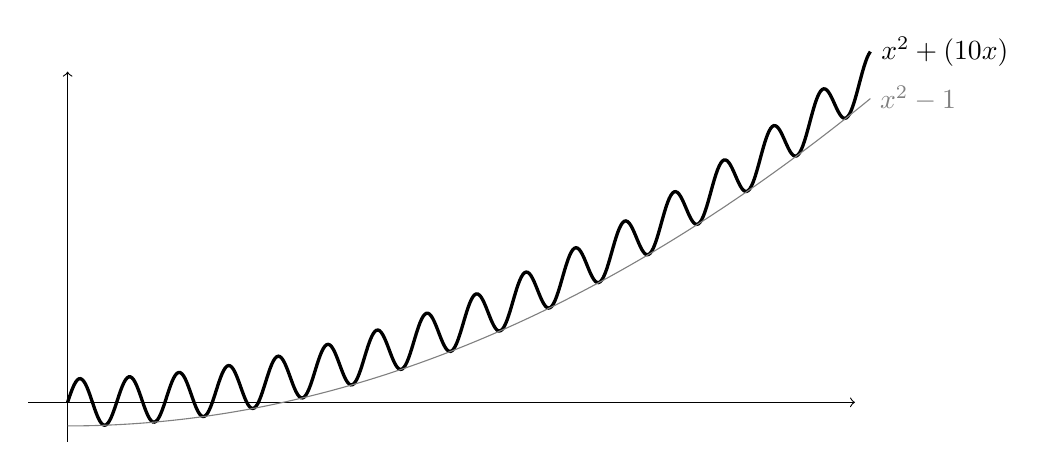
\begin{tikzpicture}
\draw[->] (-0.5,0)--(10,0);
\draw[->] (0,-0.5)--(0,4.2);
%\draw[dotted] (0.5,0) node[below]{$10$}--(0.5,0.25);
%\draw[dotted] (0,0.25) node[left]{$100$}--(2,0.25);
\draw [very thick, domain=0:10.2, samples=500] plot
(\x,{0.04*\x^2+0.3*sin(10*\x r)}) node[right]{$x^2+\sen(10x)$};
\draw [color=gray, domain=0:10.2, samples=500] plot
(\x,{0.04*\x^2-0.3}) node[right]{$x^2-1$};
\end{tikzpicture}\end{bmlimage}
\end{center}
\end{ex}

Vimos que, dependendo da base, as exponenciais e os
logaritmos possuem comportamentos diferentes no infinito. Se a base
for $a>1$,
\begin{equation}\label{eq_Lim_expinf_a} 
\boxed{
\lim_{x\to\infty}a^x=+\infty\,,\quad \quad
\lim_{x\to-\infty}a^x=0\,.
}
\end{equation}
Em particular,
\begin{equation}\label{eq_Lim_expinf_b} 
\boxed{
\lim_{x\to\infty}e^x=+\infty\,,\quad \quad
\lim_{x\to-\infty}e^x=0\,.
}
\end{equation}
Por outro lado, se a base
for $a<1$,
\begin{equation}\label{eq_Lim_expinf_c} 
\boxed{
\lim_{x\to\infty}a^x=0\,,\quad \quad
\lim_{x\to-\infty}a^x=+\infty\,.
}
\end{equation}

Os logaritmos, por sua vez,
\eq{
\boxed{
\lim_{x\to\infty}\log_ax=
\begin{cases}
 +\infty&\text{ se $a>1$,}\\
-\infty&\text{ se $a<1$.}
\end{cases}
}
}
Observe que ``$\lim_{x\to-\infty}\log_ax$'' não faz sentido, já que
o domínio de $\log_a$ é $(0,\infty)$!

\begin{exo}
Mostre que se $\lim_{x\to\infty}f(x)=\pm\infty$, então
\[ 
\lim_{x\to\infty}\frac{1}{f(x)}=0\,.
\]
\begin{sol}
Seja $\epsilon>0$. Queremos mostrar que $|\frac{1}{f(x)}|\leq \epsilon$ para todo
$x$ suficientemente grande. Como $\lim_{x\to\infty}f(x)=\pm\infty$, sabemos que
se $A=\tfrac1\epsilon$, então existe $N$ tal que $f(x)\geq A$ para todo $x\geq
N$ (em particular, $f(x)>0$ para esses $x$). Mas isso implica também
$\frac{1}{f(x)}\leq \frac{1}{A}=\epsilon$, o que queríamos. 
\end{sol}
\end{exo}

A propriedade provada no último exercício permite obter o
comportamento no infinito para as potências negativas: 
$x^{-q}=\tfrac1{x^q}$, com $q>0$. Como
$\lim_{x\to\infty}x^q=+\infty$, 
temos 
\[ 
\lim_{x\to \infty}\frac{1}{x^q}=0\,.
\]
O limite $x\to -\infty$ se calcula da mesma maneira.

\begin{exo}\label{utilparaimproprias}
Mostre que 
\[
\lim_{L\to\infty}\frac{1}{L^{1-p}}=
\begin{cases}
0&\text{ se }p<1\,,\\
1&\text{ se }p=1\,,\\
\infty&\text{ se }p>1\,.
\end{cases}
\]
%\begin{sol}
%Se $p=1$ então $\frac{1}{L^{1-p}}=1$ para todo $L>0$. 
%Os casos $p<1$ e $p>1$ se deduzem de \eqref{eq:infiniUM} e
%\eqref{eq:infiniDOIS}.
%\end{sol}
\end{exo}

É importante notar que em geral, as propriedades descritas na
Proposição \ref{Prop:SomasProdLimInfinito} 
\emph{não se aplicam} quando os limites envolvidos
são infinitos. 
Aparece frequentemente de ter que lidar com quocientes
$\frac{f(x)}{g(x)}$ ou diferenças $f(x)-g(x)$, em que ambos
$f(x)\to\infty$ e $g(x)\to\infty$. Neste caso, as identidades da
Proposição \ref{Prop:SomasProdLimInfinito} não se aplicam, e um estudo 
caso a caso é preciso.

\subsubsection{Produtos de números grandes}
Na propriedade \eqref{eq:proprliminfty2},
insistimos sobre o fato dos dois limites
$\lim_{x\to\infty}f(x)$  e $\lim_{x\to\infty}g(x)$ existirem e serem
\emph{finitos} para poder escrever
\begin{equation}\label{eq_mmjj}
\lim_{x\to\infty}\{f(x)\cdot g(x)\}=
\bigl(\lim_{x\to\infty}f(x)\bigr)\cdot\bigl(\lim_{x\to\infty}g(x)\bigr)\,.
\end{equation}
É importante entender que existem casos em que essa relação \emph{não}
pode ser usada.\\

%\begin{ex} 
Considere  $f(x)=x$, $g(x)=\frac{1}{x}$. Neste caso, $f(x)g(x)=1$,
portanto o lado esquerdo de 
\eqref{eq_mmjj} é igual a
\[ 
\lim_{x\to\infty}\{f(x)\cdot g(x)\}=
\lim_{x\to\infty}1=1\,.
\]
Mas o lado direito  é igual a
\[ 
\bigl(\lim_{x\to\infty}f(x)\bigr)\cdot\bigl(\lim_{x\to\infty}g(x)\bigr)=\infty\cdot
0\,.
\]
Portanto, se \eqref{eq_mmjj} fosse verdadeira, teríamos 
\[``1=\infty\cdot 0"\,,\]
o que já mostra que há um problema: zero multiplicado por outra coisa
dificilmente pode dar $1$...
Mas, se agora $f(x)=2x$, $g(x)=\frac1x$, então $f(x)g(x)=2$, e 
o mesmo raciocíno leva a 
\[``2=\infty\cdot 0"\,.  \]
Ou, com $f(x)=x^2$ e $g(x)=\frac1x$,
\[``\infty=\infty\cdot 0"\,.\]
Sabemos que qualquer número multiplicado por zero dá zero, mesmo se o número for
grande:
\[ 
0\cdot 10=0\,,\quad\quad
0\cdot 100=0\,,\quad\quad
0\cdot 10000000=0\,,\quad\quad
\text{ etc.}
\]
Mas os exemplos acima mostram que há um problema com 
``$0\cdot\infty$'', e 
lembram que ``$\infty$'' não pode ser manuseado como os
outros números reais: em geral ``$0\cdot \infty$'' não vale zero, e
pode valer qualquer coisa. 
É por isso que será sempre escrito usando aspas.
A gente chama ``$\infty\cdot 0$'' (ou ``$0\cdot \infty$'') 
de \grasA{forma indeterminada}.
%\end{ex}

Em termos de limites, o exemplo acima 
mostra que não se pode aplicar \eqref{eq_mmjj}
quando um dos limites é infinito e o outro zero. No entanto, 

\begin{pro}\label{prop_LIM_produtouminfinito}
Se $\lim_{x\to\infty}f(x)=+\infty$ e $\lim_{x\to\infty}g(x)=\ell$, 
$\ell\neq 0$, então 
\[ 
\lim_{x\to\infty}\{f(x)\cdot g(x)\}=
\begin{cases}
+\infty&\text{ se }\ell>0\,,\\
-\infty&\text{ se }\ell<0\,.\\
\end{cases}
\]
\end{pro}

\begin{ex}
Por exemplo, 
já que $\lim_{x\to\infty}\frac{x}{x+2}=1>0$ e $\lim_{x\to\infty}e^x=+\infty$, 
\[ 
\lim_{x\to\infty}\frac{xe^x}{x+2}=
\lim_{x\to\infty}\frac{x}{x+2}\cdot e^x=+\infty\,.
\]
\end{ex}

\subsubsection{Quocientes de números grandes}

No Exemplo \ref{Ex:razaosimples} calculamos 
$\lim_{x\to \infty}\frac{x}{x+2}=1$. Observe que 
este limite é da forma
\[ 
\lim_{x\to \infty}\frac{f(x)}{g(x)}\,,
\]
em que $\lim_{x\to\infty}f(x)=\infty$ e 
$\lim_{x\to\infty}g(x)=\infty$.
Portanto, podemos dizer que é uma \grasA{forma indeterminada}
\[ ``\frac{\infty}{\infty}"\,.
\]
Em geral, ter uma \emph{indeterminação} (qualquer que seja) não significa
que o limite considerado não existe ou que ele não pode ser calculado, mas
que um estudo mais minucioso é necessário.
De fato, os exemplos a seguir 
são todos limites da forma ``$\frac{\infty}{\infty}$'',
mas todos podem ser calculados explicitamente e dar valores
diferentes:
\[ 
\lim_{x\to\infty}\frac{x}{x^2}=0\,,\quad
\lim_{x\to\infty}\frac{x^2}{x^2}=1\,,\quad
\lim_{x\to\infty}\frac{x^3}{x^2}=\infty\,,\,\text{ etc.}
\]
\begin{obs}
Na verdade as indeterminações da forma ``$\frac{\infty}{\infty}$'' são
equivalentes às indeterminações da forma ``$\infty\cdot 0$''. De fato, se 
$\lim_{x\to \infty}\frac{f(x)}{g(x)}$ é
``$\frac{\infty}{\infty}$'', podemos escrever \[ 
\lim_{x\to \infty}\frac{f(x)}{g(x)}=
\lim_{x\to \infty}\Bigl\{f(x)\cdot \frac{1}{g(x)}\Bigr\}\,.
\]
Como 
$\lim_{x\to\infty}f(x)=\infty$ e 
$\lim_{x\to\infty}\frac{1}{g(x)}=0$, o limite acima é também da forma
``$\infty\cdot 0$''.
\end{obs}

No próximos exemplos mostraremos várias técnicas que permitem resolver
indeterminações do tipo ``$\frac{\infty}{\infty}$''.
Começaremos com razões de polinômios, em que os polinômios têm o mesmo grau.
\begin{ex} Calcularemos um limite parecido com o 
do Exemplo \ref{Ex:razaomuitosimples}:
\[\lim_{x\to\infty}\frac{3x-5}{x+2}\,.\]
É fácil mostrar que esse limite é igual a $3$, mas paremos para pensar
de uma maneira diferente.  Na fração acima, quando $x$ é grande, 
o numerador $3x-5$ e o denominador $x+2$ são ambos grandes.
No entanto quando $x$ for grande, 
no numerador o ``$-5$'' se torna desprezível comparado com o ``3x'', e 
no denominador o ``$+2$'' 
se torna desprezível comparado com o ``$x$''.
Portanto, para $x$ grande, gostaríamos de pensar que
$$
\frac{3x-5}{x+2}\quad\text{ pode ser aproximado por } 
\quad\frac{3x}{x}\,, \quad \text{ que (após simplificação) é igual a }3\,.
$$
Esse argumento não é perfeitamente rigoroso, mas 
sugere que o limite é $3$. Para tornar ele 
mais rigoroso, colocamos $x$ em evidência no
denominador, e \emph{simplificamos por $x$}:
\begin{equation}\label{eq_simplicacao}
\frac{3x-5}{x+2}=\frac{x(3-\frac5x)}{x(1+\frac{2}{x})}
=\frac{3-\frac5x}{1+\frac{2}{x}}\,.
\end{equation}
Isso é só um outro jeito de reescrever a fração, mas agora observe que
quando $x\to \infty$, o limite desta última fração
não é mais da forma ``$\frac{\infty}{\infty}$''! 
Assim, usando \eqref{eq_simplicacao}, 
\eqref{eq:proprliminfty1} e \eqref{eq:proprliminfty3}:
$$
\lim_{x\to\infty}\frac{3x-5}{x+2}=
\lim_{x\to\infty}\frac{3-\frac5x}{1+\frac{2}{x}}=
\frac{\lim_{x\to\infty}(3-\frac5x)}{\lim_{x\to\infty}(1+\frac{2}{
x})}
=\frac{3-0}{1+ 0}=3\,.
$$
\end{ex}
Neste último exemplo aprendemos a extrair, em uma fração, as partes
mais importantes. Vejamos mais um exemplo.

\begin{ex}
Considere 
\[ 
\lim_{x\to\infty}\frac{x^3+1000x}{2x^3+1}\,.
\]
Vemos que tem dois termos de grau $3$, um termo de grau $1$ e um termo de
grau $0$ (aquele $+1$). O que importa, aqui, é que no limite
$x\to\infty$, os termos de grau $3$ vão ser os mais importantes.
De fato, quando $x$ for grande, $x^3$ sendo $x\cdot x\cdot x$, será muito maior
que $x$. Logo, vamos
\emph{extrair os termos de grau $3$ no numerador e
denominador}, simplificar, e 
usar \eqref{eq:proprliminfty1}-\eqref{eq:proprliminfty3}:
\[ 
\lim_{x\to\infty}\frac{x^3+1000x}{2x^3+1}=
\lim_{x\to\infty}\frac{x^3(1+\frac{1000}{x^2})}{x^3(2+\frac{1}{x^3})}=
\lim_{x\to\infty}\frac{1+\frac{1000}{x^2}}{2+\frac{1}{x^3}}=
\frac{\lim_{x\to\infty}(1+\frac{1000}{x^2})}{\lim_{x\to\infty}(2+\frac{1}{x^3})}=
\frac{1+0}{2+0}=\frac{1}{2}\,.
\]
\end{ex}

Extrair os termos de grau maior no numerador e
denominador pode ser feito em outras situações, com potências que não são
inteiras.
\begin{ex}
Considere
\[
\lim_{x\to\infty}\frac{x^5-x^2+1}{2x^5+3\sqrt{x}}\,.
\]
O limite é da forma ``$\frac{\infty}{\infty}$'', e a fração contem termos de
grau $5$, $2$, $\tfrac12$ e $0$.
Extraindo o termo de grau maior,
\[
\frac{x^5-x^2+1}{2x^5+3\sqrt{x}}
=\frac{x^5(1-\frac{1}{x}+\frac{1}{x^5})}{x^5(2+\frac{3}{x^{9/2}})}
=\frac{1-\frac{1}{x}+\frac{1}{x^5}}{2+\frac{3}{x^{9/2}}}\,,
\]
o limite do novo quociente \emph{não é mais indeterminado}. De fato, 
o novo numerador satisfaz
$\lim_{x\to\infty}(1-\frac{1}{x}+\frac{1}{x^5})=1-0+0=1$, e o
denominador 
$\lim_{x\to\infty}(2+\frac{3}{x^{9/2}})=2+0=2$, que é diferente de zero.
Logo, por \eqref{eq:proprliminfty3},
\[
\lim_{x\to\infty}\frac{x^5-x^2+1}{2x^5+3\sqrt{x}}
=\frac{\lim_{x\to\infty}(1-\frac{1}{x}+\frac{1}{x^5})}{\lim_{x\to\infty}(2+\frac{3}{x^{9/2}})}
=\frac{1}{2}\,.
\]
\end{ex}

Vejamos agora dois exemplos em que o denominador e o numerador tem graus
diferentes.

\begin{ex}
Considere o seguinte limite, da forma ``$\fracinfty$'':
\[ \lim_{x\to\infty}\frac{x+2x^2}{1+x^4}\,.
\]
Extraindo os termos de grau maior em cima e em baixo,
\[ 
\frac{x+2x^2}{1+x^4}=
\frac{x^2(2+\frac{1}{x})}{x^4(1+\frac{1}{x^4})}=
\frac{1}{x^2}\cdot \frac{2+\frac1{x}}{1+\frac{1}{x^4}}
\]
Logo, como $\lim_{x\to\infty}\frac{1}{x^2}=0$ e
$\lim_{x\to\infty}\frac{2+\frac1x}{1+\frac{1}{x^4}}=2$, 
\eqref{eq:proprliminfty2} implica
\[ 
 \lim_{x\to\infty}\frac{x+2x^2}{1+x^4}=0\cdot 2=0\,.
\]
\end{ex}

\begin{ex}
Estudemos agora 
\[\lim_{x\to \infty}\frac{x^2+2}{x+1}\,,\]
que representa também uma indeterminação do tipo ``$\fracinfty$''.
Mas, pondo os termos de grau $2$ em evidência,
$$\frac{x^2+2}{x+1}=\frac{x^2(1+\frac{2}{x^2})}{x(1+\frac{1}{x})}=
x\cdot \frac{1+\frac{2}{x^2}}{1+\frac{1}{x}}\,.$$
Observe agora que o primeiro fator, $x$, tende a $+\infty$, e que o 
segundo fator,
$\frac{1+\frac{2}{x^2}}{1+\frac{1}{x}}$, tende a $1$. Logo, 
pela Proposição \ref{prop_LIM_produtouminfinito},
$$\lim_{x\to\infty}\frac{x^2+2}{x+1}=
\lim_{x\to\infty}x\cdot \frac{1+\frac{2}{x^2}}{1+\frac{1}{x}}=
+\infty\,.$$
\end{ex}


\begin{exo}\label{Exo:limitesinfini} Calcule os limites abaixo,
evitando o uso da 
definição formal. Abaixo, $x\to \pm\infty$ significa que são dois limites
para calcular: $x\to+\infty$ e $x\to-\infty$.
\begin{multicols}{3}
\begin{enumerate}
\item\label{itexliminfini2} $\lim_{x\to
\pm\infty}\{\frac{1}{x}+\frac{1}{x^2}+\frac{1}{x^3}\}$
\item\label{itexliminfini3} $\lim_{x\to \pm\infty}\frac{x^2-1}{x^2}$
\item\label{itexliminfini6} $\lim_{x\to\pm\infty}\frac{1-x^2}{x^2-1}$
\item\label{itexliminfini7} $\lim_{x\to
\pm\infty}\frac{2x^3+x^2+1}{x^3+x}$
\item\label{itexliminfini8} $\lim_{x\to
\pm\infty}\frac{2x^3-2}{x^4+x}$
\item\label{itexliminfini9} $\lim_{x\to\infty}\frac{1+x^4}{x^2+4}$
\item\label{itexliminfini10} $\lim_{x\to
\pm\infty}\frac{\sqrt{x+1}}{\sqrt{x}}$
\item\label{itexliminfini15}
$\lim_{x\to\pm\infty}\frac{\sqrt{4x^2+1}}{x}$
\item\label{itexliminfini11}
$\lim_{x\to\infty}\frac{3x+2}{\sqrt{x^2+3}-4}$
\item\label{itexliminfini12} $\lim_{x\to\pm\infty}
\frac{\sqrt{x+\sqrt{x+\sqrt{x}}}}{\sqrt{x+1}}$
\item\label{itexliminfini13} $\lim_{x\to\pm\infty}\frac{|x|}{x^2+1}$
\item\label{itexliminfini14} $\lim_{x\to\pm\infty}\sqrt{x^2+1}$
\item\label{itexliminfini141} $\lim_{x\to\pm\infty}\frac{1}{2^x}$
\item\label{itexliminfini16}
$\lim_{x\to\pm\infty}\frac{e^x+100}{e^{-x}-1}$
\item\label{itexliminfini161} $\lim_{x\to \pm \infty}\ln(1+\frac{x+1}{x^2})$
\item\label{itexliminfini162} $\lim_{x\to \pm \infty}\frac{\ln(1+e^x)}{x}$
\item\label{itexliminfini5} $\lim_{x\to\pm \infty}e^{\frac{1}{x}}$
\item\label{itexliminfini17} $\lim_{x\to \pm\infty}\sen^2x$
\item\label{itexliminfini19} $\lim_{x\to \pm\infty}\arctan x$
\item\label{itexliminfini20} $\lim_{x\to \pm\infty}\senh x$
\item\label{itexliminfini21} $\lim_{x\to \pm\infty}\cosh x$
\item\label{itexliminfini22} $\lim_{x\to \pm\infty}\tanh x$
\end{enumerate}
\end{multicols}
\vspace{0.01cm}
\begin{sol}
\eqref{itexliminfini2} Como $\lim_{x\to\pm\infty}\frac{1}{x^q}=0$ para
qualquer $q>0$, usando \eqref{eq:proprliminfty1} dá 
$\lim_{x\to
\pm\infty}\{\frac{1}{x}+\frac{1}{x^2}+\frac{1}{x^3}\}=0$.
\eqref{itexliminfini3} $\lim_{x\to \pm\infty}\frac{x^2-1}{x^2}=1$
\eqref{itexliminfini6} $\lim_{x\to\pm\infty}\frac{1-x^2}{x^2-1}=-1$.
\eqref{itexliminfini7} Colocando $x^3$ em evidência e usando
\eqref{eq:proprliminfty3}, 
$$\lim_{x\to\pm\infty}\frac{2x^3+x^2+1}{x^3+x}=\lim_{x\to
\pm\infty}\frac{x^3(2+\frac{1}{x}+\frac{1}{x^3})}{x^3(1+\frac{1}{x^2})
} =\lim_{x\to
\pm\infty}\frac{2+\frac{1}{x}+\frac{1}{x^3}}{1+\frac{1}{x^2}}=\frac{2}
{1}=2\,.$$
\eqref{itexliminfini8} $\lim_{x\to
\pm\infty}\frac{2x^3-2}{x^4+x}=0$
\eqref{itexliminfini9} Colocando $x^4$ em
evidência no denominador, $x^2$ no numerador,
$\frac{1+x^4}{x^2+4}=x^2\frac{\frac{1}{x^4}+1}{1+\frac{4}{x^2}}$.
Como $x^2\to\infty$ e que a fração tende a $1$, temos 
$\lim_{x\to\pm\infty}\frac{1+x^4}{x^2+4}=\infty$.
\eqref{itexliminfini10} ``$\lim_{x\to
-\infty}\frac{\sqrt{x+1}}{\sqrt{x}}$'' não é definido.
Por outro lado, colocando $\sqrt{x}$ em evidência, 
$$\lim_{x\to+\infty}\frac{\sqrt{x+1}}{\sqrt{x}}=
\lim_{x\to +\infty}\frac{\sqrt{1+\frac{1}{{x}}}}{1}=1\,.
$$
\eqref{itexliminfini15}
Lembrando que $\sqrt{x^2}=|x|$ (Exercício
\ref{Exo:valorabscorreto}!), temos
$\frac{\sqrt{4x^2+1}}{x}=\frac{\sqrt{x^2(4+\frac{1}{x^2})}}{x}=\frac{
|x|}{x}\sqrt{4+\frac{1}{x^2}}$.
Como $\frac{|x|}{x}=+1$ se $x>0$, $=-1$ se $x<0$, temos $\lim_{x\to\pm\infty}\frac{|x|}{x}=\pm 1$. Como 
$\lim_{x\to\pm\infty}\sqrt{4+\frac{1}{x^2}}=\sqrt{4}=2$, temos
$\lim_{x\to\pm\infty}\frac{\sqrt{4x^2+1}}{x}=\pm 2$.
\eqref{itexliminfini11} 
Do mesmo jeito,
$\sqrt{x^2+3}=|x|\sqrt{1+\frac{3}{x^2}}$. Assim,
$$
\frac{3x+2}{\sqrt{x^2+3}-4}=\frac{x}{|x|}\frac{3+\frac{2}{x}}{\sqrt{1+
\frac{3}{x^2}}-\frac{4}{|x|}}
$$
Como $\lim_{x\to\pm\infty}\frac{x}{|x|}=\pm 1$, e que a razão tende a
$3$, temos 
$$\lim_{x\to+\infty}\frac{3x+2}{\sqrt{x^2+3}-4}=+3\,,\quad 
\lim_{x\to-\infty}\frac{3x+2}{\sqrt{x^2+3}-4}=-3\,.
$$
\eqref{itexliminfini12} O limite $x\to-\infty$
não é definido, e $\lim_{x\to+\infty}
\frac{\sqrt{x+\sqrt{x+\sqrt{x}}}}{\sqrt{x+1}}=1$.
\eqref{itexliminfini13} $\lim_{x\to\pm\infty}\frac{|x|}{x^2+1}=0$
\eqref{itexliminfini14} $\lim_{x\to\pm\infty}\sqrt{x^2+1}=+\infty$
\eqref{itexliminfini141} Como $\frac{1}{2^x}=2^{-x}$, temos $\lim_{x\to+\infty}\frac{1}{2^x}=0$, 
$\lim_{x\to-\infty}\frac{1}{2^x}=+\infty$.
\eqref{itexliminfini16}
$\lim_{x\to+\infty}\frac{e^x+100}{e^{-x}-1}=-\infty$,
$\lim_{x\to-\infty}\frac{e^x+100}{e^{-x}-1}=0$.
\eqref{itexliminfini161}  Primeiro mostre (usando os mesmos métodos do que os que foram
usados nos outros itens) que $\lim_{x\to \pm \infty}(1+\frac{x+1}{x^2})=1$. Em seguida,
observe que 
se $z$ se aproxima de $1$,  então $\ln(z)$ se aproxima de $\ln(1)=0$. Logo, $\lim_{x\to
\pm \infty}\ln(1+\frac{x+1}{x^2})=0$. Obs: dizer que ``se $z$ se aproxima de $1$, então
$\ln(z)$ se aproxima de $\ln(1)$'' presupõe que a função $\ln$ é \emph{contínua} em $1$.
Continuidade será estudada no fim do capítulo.
\eqref{itexliminfini162}  Escreve $(1+e^x)=e^x(1+e^{-x})$, logo
$\frac{\ln(1+e^x)}{x}=\frac{\ln
e^x}{x}+\frac{\ln(1+e^{-x})}{x}=1+\frac{\ln(1+e^{-x})}{x}$. Mas $\lim_{x\to
\infty}\frac{\ln(1+e^{-x})}{x}=0$, logo
$\lim_{x\to \infty}\frac{\ln(1+e^{x})}{x}=1$.
Por outro lado, $\ln(1+e^x)\to 0$  quando $x\to-\infty$, logo $\lim_{x\to
-\infty}\frac{\ln(1+e^{x})}{x}=0$.
\eqref{itexliminfini5} Como $\lim_{x\to\pm \infty}\frac{1}{x}=0$
temos, $\lim_{x\to\pm \infty}e^{\frac{1}{x}}=e^0=1$.
\eqref{itexliminfini17} $``\lim_{x\to \pm\infty}\sen^2x''$ não existe.
\eqref{itexliminfini19} $\lim_{x\to \pm\infty}\arctan
x=\pm\pisobredois$.
\eqref{itexliminfini20} 
Por definição, $\senh x=\frac{e^x-e^{-x}}{2}$. Para estudar
$x\to\infty$, coloquemos $e^x$ em evidência:
$\frac{e^x-e^{-x}}{2}=e^x\frac{1-e^{-2x}}{2}$. Como $e^x\to\infty$ e
$1-e^{-2x}\to 1$ temos $\lim_{x\to \infty}\senh x=+\infty$. Como
$\senh x$ é ímpar, temos $\lim_{x\to -\infty}\senh x=-\infty$.
\eqref{itexliminfini21} $\lim_{x\to \pm\infty}\cosh x=+\infty$
\eqref{itexliminfini22} Para estudar, $x\to\infty$:
$\tanh x=\frac{e^x-e^{-x}}{e^x+e^{-x}}=\frac{e^x}{e^x}\frac{1-e^{-2x}}{1+e^{
-2x }}=\frac{1-e^{-2x}}{1+e^{
-2x }}$, logo $\lim_{x\to +\infty}\tanh x=+1$. Como $\tanh$ é ímpar,
$\lim_{x\to -\infty}\tanh x=-1$.
\end{sol}
\end{exo}



\begin{exo}
% http://limite.cours-de-math.eu/solution-probleme2.php
Um tempo $t$ depois de ter pulado do avião, a velocidade
vertical de um paraquedista em queda livre é dada por:
$$V(t)=\sqrt{\frac{m g}{k}}\tanh\Bigl(\sqrt{\frac{gk}{m}}t\Bigr)\,,$$
onde $m$ é a massa do paraquedista, $g=9,81m/s^2$, e $k$ é um
coeficiente de resistência (atrito) do ar (em $kg/m$). Esboce
$t\mapsto V(t)$,
e calcule o limite de velocidade $V_{\rm lim}$ (que ele nunca
atingirá).
Dê uma estimativa de $V_{\rm lim}$ quando $m=80kg$, $k=0.1kg/m$.
\begin{sol}
Pelo gráfico de $x\mapsto \tanh x$, vemos que $V(t)$ cresce e tende a
um valor limite, dado por 
$$
V_{\rm lim}=\lim_{t\to\infty}V(t)=\sqrt{\frac{m
g}{k}}\lim_{t\to\infty}\tanh\Bigl(\sqrt{\frac{gk}{m}}t\Bigr)
$$
Vimos no Exercício \ref{Exo:limitesinfini} que
$\lim_{x\to\infty}\tanh x=1$. Portanto, 
$$V_{\rm lim}=\sqrt{\frac{m
g}{k}}\,.$$
Observe que $V(t)<V_{\rm lim}$ para todo $t$, então o paraquedista
nunca atinge a velocidade limite, mesmo se ele cair um tempo infinito!
Com os valores propostos,
$V_{\rm lim}=\sqrt{80\cdot 9,81/0.1}\simeq 89m/s\simeq 318km/h$.
\end{sol}
\end{exo}

\subsubsection{Somas e diferenças de números grandes}

Na propriedade \eqref{eq:proprliminfty1},
insistimos sobre o fato dos dois limites
$\lim_{x\to\infty}f(x)$  e $\lim_{x\to\infty}g(x)$ serem
\emph{finitos} para poder escrever
$$\lim_{x\to\infty}\{f(x)+g(x)\}=
\lim_{x\to\infty}f(x)+\lim_{x\to\infty}g(x)\,.$$

Quando os dois limites são infinitos, com o mesmo sinal, então o
limite da soma pode também ser calculado:

\begin{ex}
Considere $x+x^3$. Como $\lim_{x\to\infty}x=+\infty$ e
$\lim_{x\to\infty}x^3=+\infty$ (aqui, ambos tem o sinal ``$+$''), temos 
$\lim_{x\to\infty}\{x+x^3\}=+\infty$.
\end{ex}

Agora, para estudar $\lim_{x\to\infty}\{f(x)-g(x)\}$, com
$\lim_{x\to\infty}f(x)=\infty$ e
$\lim_{x\to\infty}g(x)=\infty$, 
leva a um caso de \grasA{indeterminação do
tipo ``$\infty-\infty$''}. Vejamos exemplos que ilustram que de
fato, ``$\infty-\infty$'' pode tomar qualquer valor.

\begin{ex}
Considere $x^3-x^2$, em que $\lim_{x\to\infty}x^3=+\infty$ e
$\lim_{x\to\infty}x^2=+\infty$. Como o termo de grau
maior deve ser mais importante, escrevamos
$x^3-x^2=x^3(1-\frac{1}{x})$. Como $x^3\to\infty$ e
$1-\frac{1}{x}\to 1$, a Proposição \ref{prop_LIM_produtouminfinito} 
garante que 
\[\lim_{x\to\infty}\{x^3-x^2\}=+\infty\,.\]
O que aconteceu aqui se resume assim: $x^3$ e $x^2$ ambos tendem a
$+\infty$, mas $x^3$ \emph{cresce mais rápido} que $x^2$, e isso
implica que a diferença $x^3-x^2$ é regida (quando $x$ é grande)
pelo termo $x^3$.
\end{ex}

\begin{ex}
A diferença $x^2-x^4$ no limite $x\to\infty$ pode ser estudada da
mesma maneira: $x^2-x^4=x^4(\frac{1}{x^2}-1)$, e como $x^4\to\infty$,
$(\frac{1}{x^2}-1)\to-1$, temos que $x^2-x^4\to -\infty$.
Aqui, é o termo $-x^4$ que rege o comportamento para $x$ grande.
\end{ex}


\begin{ex}\label{Ex:conjugadobasico}
Considere $\sqrt{x+1}-\sqrt{x}$. Quando $x\to\infty$, os dois termos
$\sqrt{x+1}$ e $\sqrt{x}$ tendem a $+\infty$, mas eles são do mesmo grau. 
\index{indeterminação!do tipo ``$\infty-\infty$''}
Como calcular o limite dessa diferênça? O método usado aqui consiste em
\emph{multiplicar e
dividir pelo \index{conjugado}conjugado}, isto é, escrever ``$1$'' como
$$
1=\frac{\sqrt{x+1}+\sqrt{x}}{
\sqrt{x+1}+\sqrt{x}}\,.
$$
Lembrando que $(a-b)(a+b)=a^2-b^2$,
$$
\sqrt{x+1}-\sqrt{x}=(\sqrt{x+1}-\sqrt{x})\frac{\sqrt{x+1}+\sqrt{x}}{
\sqrt{x+1}+\sqrt{x}}=\frac{\sqrt{x+1}^2-\sqrt{x}^2}{\sqrt{x+1}+\sqrt{
x}}=\frac{1}{\sqrt{x+1}+\sqrt{x}}\,.
$$
Mas como $\sqrt{x+1}+\sqrt{x}\to\infty$, temos
$$\lim_{x\to\infty}\{\sqrt{x+1}-\sqrt{x}\}=\lim_{x\to\infty}\frac{1}{
\sqrt{x+1}+\sqrt{x}}=0\,.$$ 
\end{ex}

\begin{exo}
Calcule os limites quando $x\to\infty$ das seguintes funções.
\begin{multicols}{3}
\begin{enumerate}
\item\label{itexliminfini1} $7-x$
\item\label{itexliminfini4} $\sqrt{1-x}$
\item\label{itexliminfini18} $x+\cos x$
\item\label{itexoinfinf1} $100x-x^2$
\item\label{itexoinfinf2} $x^7-x^7$
\item\label{itexoinfinf3} $x^4-\tfrac12 x^4$
\item\label{itexoinfinf311} $(x-1)^2-x^2$
\item\label{itexoinfinf31} $x-\sqrt{x}$
\item\label{itexoinfinf5} $\sqrt{x^2+1}-\sqrt{x^2-x}$
\item\label{itexoinfinf51} $\sqrt{x^2+1}-\sqrt{x^2-3x}$
\item\label{itexoinfinf4} $\sqrt{2x}-\sqrt{x+1}$
\item\label{itexoinfinf6} $e^x-e^{2x}$
\item\label{itexoinfinf7} $\ln(x)-\ln(2x)$
\item\label{itexoinfinf8} $\ln(x)-\ln(x+1)$
\end{enumerate}
\end{multicols}
\vspace{0.01cm}
\begin{sol}
\eqref{itexliminfini1} $\lim_{x\to\infty}(7-x)=-\infty$,
$\lim_{x\to-\infty}(7-x)=+\infty$.
\eqref{itexliminfini4} ``$\lim_{x\to +\infty}\sqrt{1-x}$'' não é
definida, pois o domínio de $\sqrt{1-x}$ é $(-\infty,1]$. 
$\lim_{x\to -\infty}\sqrt{1-x}=+\infty$.
\eqref{itexliminfini18} Como $\lim_{x\to\pm\infty}
x=\pm\infty$, e que $\cos x$ é limitado por $-1\leq \cos x\leq 1$,
temos $\lim_{x\to \pm\infty}x+\cos x=\pm\infty$.
\eqref{itexoinfinf1} $-\infty$.
\eqref{itexoinfinf2} $0$.
\eqref{itexoinfinf3} $+\infty$.
\eqref{itexoinfinf311} $-\infty$
\eqref{itexoinfinf31} $+\infty$
\eqref{itexoinfinf5} $\frac12$.
Esse ítem (e o próximo) mostram que argumentos informais do tipo
``$x^2+1\simeq x^2$
quando $x$ é grande'' não sempre são eficazes! De fato, aqui daria
$\sqrt{x^2+1}-\sqrt{x^2-x}\simeq \sqrt{x^2}-\sqrt{x^2}=0$...
\eqref{itexoinfinf51} $\frac32$. 
\eqref{itexoinfinf4} Aqui não precisa multiplicar pelo conjugado: pode
simplesmente colocar $\sqrt{x}$ em evidência:
$\sqrt{2x}-\sqrt{x+1}=\sqrt{x}(\sqrt{2}-\sqrt{1+\frac1x})$. Como
$\sqrt{x}\to\infty$ e $\sqrt{2}-\sqrt{1+\frac1x}\to \sqrt{2}-1>0$,
temos $\sqrt{x}(\sqrt{2}-\sqrt{1+\frac1x})\to +\infty$.
\eqref{itexoinfinf6} $-\infty$ (Obs: pode observar que $e^x-e^{2x}=z-z^2$, em que $z=e^x$. Como $z\to \infty$ 
quando $x\to\infty$, temos $z-z^2\to \infty$, como no item \eqref{itexoinfinf1}.)
\eqref{itexoinfinf7} Como $\ln x-\ln(2x)=-\ln 2$, o limite é $-\ln 2$.
\eqref{itexoinfinf8} $\lim_{x\to \infty}\{\ln x-\ln(x+1)\}=
\lim_{x\to \infty}\ln (\frac{x}{x+1})=\ln 1=0$.
\end{sol}
\end{exo}

\subsubsection{O ``sanduiche''}
\index{``sanduíche''}
\begin{ex}\label{ex_LIM_sinxsurx}
Considere o limite
$\lim_{x\to \infty}\frac{\sen x}{x}$.
Sabemos que o denominador tende a $+\infty$, mas
$\sen x$ não possui limite quando $x\to\infty$.
Apesar de tudo, sabemos que $\sen x$ é uma função \emph{limitada}:
\index{função!limitada}
para todo $x$, $-1\leq \sen x\leq +1$. Portanto, quando $x>0$, 
$$
-\frac{1}{x}\leq \frac{\sen x}{x}\leq +\frac{1}{x}\,.
$$
Mas como a cota superior $+\frac1x$ tende a zero, e que a cota
inferior $-\frac1x$ também tende a zero, a função $\frac{\sen x}{x}$ 
também deve tender a zero:
\begin{center}
\begin{bmlimage}\begin{tikzpicture}
\pgfmathsetmacro{\a}{2}
\draw [color=gray!80, domain=0.7:6, samples=100] plot
(\x,{1/(\x^1)});
\draw [color=gray!80, domain=0.7:6, samples=100] plot
(\x,{-1/(\x^1)});
\draw [ ->] (-0.1,0)--(6.5,0);
\draw [ ->] (0,-1.4)--(0,1.4);
\draw [thick, domain=0.7:6, samples=100] plot
(\x,{sin(3*\x r)/\x});
\pgfmathsetmacro{\b}{2};
\draw[color=gray!90,<-] (\b,{1/\b+0.1})--(\b+0.7,{1/\b+0.7})
node[right]{$+\tfrac{1}{x}$};
\draw[color=gray!90,<-] (\b,{-1/\b-0.1})--(\b+0.7,{-1/\b-0.7})
node[right]{$-\tfrac{1}{x}$};
\draw[<-] (3.1,{0.1})--(3.7,0.8)
node[right]{$\tfrac{\sen x}{x}$};
\draw (11,0.5) node[left]{$\displaystyle{\Rightarrow \lim_{x\to
\infty}\frac{\sen x}{x}=0}$};
\end{tikzpicture}\end{bmlimage}
\end{center}
\end{ex}

Esse método vale em geral:

\begin{teo}\label{Teo:Sanduicheinfinito}
 Suponha que $f$, $g$ e $h$ seja três funções que satisfazem
$$
g(x)\leq f(x)\leq h(x)\,,\text{ para todo $x$ suficientemente grande.}
$$
Suponha também que
$\lim_{x\to\infty}g(x)=\lim_{x\to\infty}h(x)=\ell$. Então 
$\lim_{x\to\infty}f(x)=\ell$.
\end{teo}



\begin{exo} Calcule:
\begin{multicols}{3}
\begin{enumerate}
\item\label{itexosanduiche2}
$\lim_{x\to\infty}\frac{1+\cos(x^2+3x)}{x^2}$
\item\label{itexosanduiche1} $\lim_{x\to\infty}\frac{x+\sen x}{x-\cos
x}$
\item\label{itexosanduiche3} $\lim_{x\to\infty}e^{-x}\sen x$
\item\label{itexosanduiche4}
$\lim_{x\to\infty}\frac{x-\lfloor x\rfloor}{x}$
\item\label{itexosanduiche5}
$\lim_{x\to \infty}\frac{\arctan(\sen x)}{\ln x}$
\item\label{itexosanduiche6}
$\lim_{x\to\infty}\bigl\{1+\frac{\sen x}{x^2+4}\bigr\}$
\end{enumerate}
\end{multicols}
\vspace{0.01cm}
\begin{sol}
\eqref{itexosanduiche2} Para todo $x$, $-1\leq
\cos(x^2+3x)\leq +1$, logo
$0\leq \frac{1+\cos(x^2+3x)}{x^2}\leq \frac{2}{x^2}$.
Como $\frac{2}{x^2}$ tende a zero,
$\lim_{x\to\infty}\frac{1+\cos(x^2+3x)}{x^2}=0$.
\eqref{itexosanduiche1} Como $\frac{x+\sen x}{x-\cos
x}=\frac{1+\frac{\sen x}{x}}{1-\frac{\cos x}{x}}$, e como
$\lim_{x\to\infty}\frac{\sen x}{x}=0$, $\lim_{x\to\infty}\frac{\cos
x}{x}=0$ (mesmo método), temos que $\lim_{x\to\infty}\frac{x+\sen
x}{x-\cos x}=1$.
\eqref{itexosanduiche3} 
Como $-e^{-x}\leq e^{-x}\sen x\leq e^{-x}$ e 
$\lim_{x\to\infty}-e^{-x}=\lim_{x\to\infty}e^{-x}=0$, o limite
procurado vale $0$.
\eqref{itexosanduiche4} Como $0\leq x-\lfloor x\rfloor\leq 1$, temos
$\lim_{x\to\infty}\frac{x-\lfloor x\rfloor}{x}=0$.
\eqref{itexosanduiche5} Como
$-\frac{\pi/2}{\ln x}\leq \frac{\arctan(\sen x)}{\ln x}\leq
\frac{\pi/2}{\ln x}$, e $\lim_{x\to\infty}\frac{1}{\ln x}=0$, o
limite procurado é $0$.
\eqref{itexosanduiche6} Para todo $x$,
$-\frac{1}{x^2+4}\leq \frac{\sen x}{x^2+4}\leq
\frac{1}{x^2+4}$. Como 
$\lim_{x\to \infty}\frac{1}{x^2+4}=0$, o limite procurado vale
$1$.
\end{sol}
\end{exo}


\begin{obs}
Alguns limites no infinito, tais como
$\lim_{x\to \infty}\frac{e^x}{x}$  ou  $\lim_{x\to \infty} \frac{\ln x}{x}$,
não podem ser calculados com os métodos desenvolvidos até agora; serão estudados mais tarde.
\end{obs}

% \subsubsection{Assíntotas oblíquas}
% 
% Quando uma função possui uma assíntota, é uma especie de
% simplificação do comportamento: é essencialmente uma reta...

\section{Limites laterais: $\lim_{x\to a^\pm}f(x)$}\label{Sec:Lim}
\index{limite!lateral}
Na seção anterior estudamos o comportamento de uma função $f$
longe da origem, $x\to\infty$ ou $x\to-\infty$. 
Agora observaremos
o comportamento de uma função $f(x)$ a medida que $x$ 
se aproxima de um ponto da reta, que denotaremos por $a\in \bR$.
\\

Como um $x$ pode estar ou à esquerda de $a$ ($x<a$), ou à direita
de $a$ ($x>a$), começaremos com dois tipos de limites, chamados de
\grasA{laterais}: escreveremos $x\to a^+$ (ou $x\searrow a$) para
indicar que $x$ se aproxima de $a$ pela direita, e 
$x\to a^-$ (ou $x\nearrow a$) para indicar que $x$ se aproxima de $a$ pela esquerda.

Comecemos com um exemplo bem simples.
\begin{ex}\label{ExemploLimitesimples}
Considere a função \[f(x)=\frac{x}{2}+1\,,\] 
em uma vizinhança do ponto $a=1$. Olhemos primeiro os
valores de $f(x)$ quando $x\searrow 1$, isto é, quando $x$ toma valores maiores mas perto
de $1$:
\begin{center}
\begin{tabular}{c|c|c|c|c}
$x=$&$1.5$&$1.1$&$1.01$&$1,0001$\\
\hline
$f(x)= $&$1.75$&$1.55$&$1.505$&$1,50005$
\end{tabular}
\end{center}
Vemos que
estes valores decrescem, se aproximando de $1.5=\tfrac32$. Gostaríamos de escrever
\[\lim_{x\searrow 1}f(x)=\tfrac32\,.\]
Ao olharmos
os valores de $f(x)$ quando $x\nearrow 1$, isto é, quando $x$ toma valores menores mas
perto de $1$, 
vemos que estes crescem para o mesmo valor $\tfrac32$: 
\begin{center}
\begin{tabular}{c|c|c|c|c}
$x=$&$0.5$&$0.9$&$0.99$&$0.9999$\\
\hline
$f(x)= $&$1.25$&$1.45$&$1.495$&$1,49995$
\end{tabular}
\end{center}
Gostariamos então de escrever
\[\lim_{x\nearrow 1}f(x)=\tfrac32\,.\]
Essas propriedades se tornam óbvias olhando para o gráfico, que é uma simples reta:
\begin{center}
\begin{bmlimage}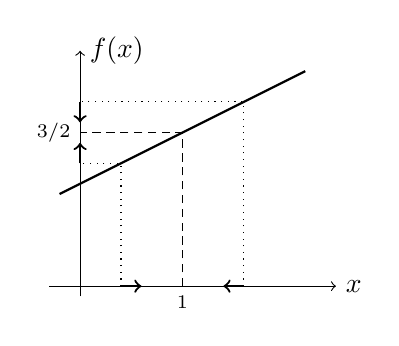
\begin{tikzpicture}[scale=1.3]
\draw [ ->] (0,-0.1)--(0,2.3) node[right]{$f(x)$};
\draw [ ->] (-0.3,0)--(2.5,0)  node[right]{$x$};
\draw [thick, domain=-0.2:2.2] plot (\x,{1+\x/2});
\pgfmathsetmacro{\e}{0.2};
\pgfmathsetmacro{\x}{1.6};
\draw[dotted] (\x,0) --(\x,{1+\x/2})--(0,{1+\x/2});
\draw[thick, <-] (\x-\e,0)--(\x,0);
\draw[thick, <-] (0,{1+\x/2-\e})--(0,{1+\x/2});
\pgfmathsetmacro{\x}{0.4};
\draw[dotted] (\x,0) --(\x,{1+\x/2})--(0,{1+\x/2});
\draw[thick, ->] (\x,0)--(\x+\e,0);
\draw[thick, ->] (0,{1+\x/2})--(0,{1+\x/2+\e});
\pgfmathsetmacro{\x}{1};
\draw[densely dashed] (\x,0) node[below]{$\scriptstyle{1}$}--(\x,{1+\x/2})--(0,{1+\x/2})
node[left]{$\scriptstyle{3/2}$};
\end{tikzpicture}\end{bmlimage}
\end{center}
Para entender um pouco melhor o que está acontecendo, vamos 
estudar a diferença:
\[|f(x)-\tfrac32|=\bigl|(\tfrac{x}{2}+1)-\tfrac32\bigr|=\tfrac12|x-1|\,.\]
Assim, vemos que quando $x$ fica perto de $1$, isto é quando a distância 
$|x-1|$ é
pequena, então a diferença $|f(x)-\tfrac32|$ é pequena também.
Poderíamos ser um pouco mais precisos, fixar uma \grasA{tolerância} $\epsilon>0$
(subentendido pequena) e perguntar:
\emph{quão próximo de $1$ $x$ precisa estar para garantir que }
\[|f(x)-\tfrac32|\leq
\epsilon\,\quad ?\]
Como $|f(x)-\tfrac32|=\tfrac12|x-1|$, vemos que $x$ precisa satisfazer
$\tfrac12|x-1|\leq \epsilon$, isto é
\[|x-1|\leq 2\epsilon\,.  \]
Logo, a resposta à pergunta acima é: \emph{a distância menor que $2\epsilon$.}
\end{ex}

Na verdade, 
pode parecer óbvio que a medida que $x$ se aproxima de $1$, a função
$f(x)=\frac{x}{2}+1$ se aproxima de $f(1)=\tfrac{1}{2}+1=\tfrac32$. Isto
é: colocando o valor $x=1$ na função, a
gente já sabe qual será o valor limite. 
Mas isso funciona porque a função do exemplo é simples o suficiente. Às 
vezes, teremos que trabalhar mais, como no próximo exemplo.

%É importante mencionar 
%que os limites estudados no exemplo anterior \emph{não dependem do valor da função no ponto $a=1$!}
%De fato, se $g$ for uma modificação de $f$ em $1$, por exemplo
%$$
%g(x)\pardef
%\begin{cases}
% \frac{x}{2}+1 &\text{ se }x\neq 1,\\
%0&\text{ se }x=1\,,
%\end{cases}
%$$
%então os limites laterais de $g$ em $x=1$ são os \emph{mesmos} que os de $f$, isto é:
%$\lim_{x\searrow 1}g(x)=\lim_{x\nearrow 1}g(x)=\tfrac32$.

% Vimos que a função $f(x)=\tfrac{x}{2}+1$ \emph{tende a} $\tfrac32$, isto é, que
% $|f(x)-\tfrac32|$ tende a zero, 
% quando $x$ tende a 1. 

\begin{ex}\label{Ex:primeironaotrivial} Consideremos agora 
\[f(x)=\frac{x^3-1}{x-1}\,,\]
também na vizinhança de $a=1$.
Observe que essa função \emph{não é definida em $1$}. Logo, 
para saber o que acontece quando $x$ tende a $1$, não
temos como adivinhar qual será o limite trocando simplesmente $x$ por $1$.

Mas isso não significa que ele não pode ser calculado. Calculemos alguns valores 
de $f(x)$, com $x\searrow 1$,
\begin{center}
\begin{tabular}{c|c|c|c|c}
$x=$&1.1&1.02&1.002&1.0002\\
\hline
$f(x)\simeq $&$3,310$&$3,060$&$3.006$&$3,001$
\end{tabular}
\end{center}
e quando $x\nearrow 1$:
\begin{center}
\begin{tabular}{c|c|c|c|c}
$x=$&0,9&0,99&0.999&0.9999\\
\hline
$f(x)\simeq $&$2,710$&$2,970$&$2,997$&$2,999$
\end{tabular}
\end{center}
Esses números sugerem que
\[\lim_{x\to 1^+}f(x)=\lim_{x\to 1^-}f(x)=3\,.\] 
Não falaremos de tolerância aqui, mas podemos 
fazer uma conta simples que mostra porque que o limite é $3$.
De fato, o polinômio $x^3-1$ possui a raiz $x=1$, sabemos então 
que ele pode ser fatorado da seguinte maneira:
\[ x^3-1=(x-1)(\dots)\,.
\]
O fator $(\dots)$ pode ser calculado pela divisão de $x^3-1$ por $x-1$,
que dá:
\[
\begin{array}{r|l}
x^3 \phantom{+x^2+x}-1 & x-1 \\ \cline{2-2}
x^3-x^2\phantom{+x+1} & x^2+x+1 \\ \cline{1-1} \\
x^2\phantom{+x}-1 \\
   x^2-x\phantom{-1} \\ \cline{1-1} \\
                       x - 1\\
		       x-1 \\\cline{1-1}\\
		       0
  \end{array}
\]
Isto mostra que o nosso quociente na verdade pode ser escrito como
$$\frac{x^3-1}{x-1}=x^2+x+1\,.$$
Agora fica claro que se $x$ tende a $1$, não importa de qual lado, 
\eq{\label{eq:limsombesta}
\lim_{x\to 1^\pm}\frac{x^3-1}{x-1}=
\lim_{x\to 1^\pm}(x^2+x+1)= 1^2+1+1=3\,.} 
\end{ex}

\begin{obs}
No exemplo anterior, a função $\frac{x^3-1}{x-1}$ 
não é definida \emph{no} ponto $a=1$, mas 
em qualquer outro ponto da sua vizinhança, e à medida que $x$ se aproxima de $a=1$, o
numerador e o denominador \emph{ambos} tendem a $0$. 
Foi o nosso primeiro exemplo de resolução de uma \grasA{indeterminação do tipo}
\index{indeterminação!do tipo ``$\frac00$''}
\[``\frac{0}{0}"\,.\]
\end{obs}

\begin{exo}\label{Exo_derivpotpasencore}
Calcule $\lim_{x\to 1^{\pm}}\frac{x^4-1}{x-1}$,
$\lim_{x\to 1^{\pm}}\frac{x^5-1}{x-1}$, ...
\begin{sol}
 A divisão dá $\frac{x^4-1}{x-1}=x^3+x^2+x+1$. Logo, como cada termo tende a $1$,
$\lim_{x\to 1^{\pm}}\frac{x^4-1}{x-1}=4$.
 No caso geral, $\frac{x^n-1}{x-1}=x^{n-1}+\dots+x+1$. Como são $n$ termos e que cada um
tende a $1$, temos $\lim_{x\to 1^{\pm}}\frac{x^n-1}{x-1}=n$.
\end{sol}
\end{exo}

Eis agora a definição geral de limite lateral:

\begin{defin} Seja $a\in \bR$. 
\begin{enumerate}
\item  Diz-se que \grasA{$f(x)$ tende a $\ell$ quando $x$ tende a $a$ pela direita} se
para todo $\epsilon>0$ existe um $\delta>0$
tal que se $a<x\leq a+\delta$, então $|f(x)-\ell|\leq \epsilon$.
Escreve-se $\lim_{x\to a^+}f(x)=\ell$.
\item  Diz-se que \grasA{$f(x)$ tende a $\ell$ quando $x$ tende a $a$ pela esquerda} se
para todo $\epsilon>0$ existe um $\delta>0$
tal que se $a-\delta\leq x< a$, então $|f(x)-\ell|\leq \epsilon$.
Escreve-se $\lim_{x\to a^-}f(x)=\ell$.
\end{enumerate}
\end{defin}

\begin{ex}
Usando a definição, mostremos que 
\[\lim_{x\to 1}x^2=1\,.\]
Observe primeiro que $|x^2-1|=|x+1|\cdot |x-1|$. 
Quando $x>1$ fica perto de $1$, digamos a distância menor que $\tfrac12$, temos
$|x-1|=x-1$, e $|x+1|=x+1\leq \tfrac52$. 
Quando $x$ tende a $1$, $|x-1|$ tende a
$0$. 
Seja agora $\epsilon>0$.
Para garantir que
$|x^2-1|\leq \epsilon$, podemos escrever primeiro $|x^2-1|\leq \tfrac52(x-1)$, e procurar
primeiro 
resolver $\tfrac52(x-1)\leq \epsilon$, que dá $x\leq 1+\tfrac25\epsilon$. Assim,
mostramos que se $1<x\leq 1+\delta$, com  
$\delta\pardef \frac{2\epsilon}{5}$, 
 teremos
$|x^2-1|=|x+1|\cdot |x-1|\leq \tfrac32(x-1)\leq \tfrac32\delta=\epsilon$.
\end{ex}

Foi usado implicitamente em \eqref{eq:limsombesta} que se cada termo de uma soma possui
limite, então a soma possui limite também, e este vale a soma dos limites; segue do
seguinte resultado, que é o análogo da Proposição \ref{Prop:SomasProdLimInfinito}:

\begin{pro}\label{Prop:ProprLimitesparaa}
\index{limite!propriedades}
Suponha que duas funções, $f$ e $g$,
possuam limites quando $x\to a^+$: 
$$\lim_{x\to a^+}f(x)=\ell_1\,,\quad
\lim_{x\to a^+}g(x)=\ell_2\,,$$
onde $\ell_1$ e $\ell_2$ são ambos \emph{finitos}. Então 
\begin{gather}
\lim_{x\to a^+}\{f(x)+g(x)\}=
\lim_{x\to a^+}f(x)+\lim_{x\to a^+}g(x)=\ell_1+\ell_2\,,
\label{eq:proprlima1} \\
\lim_{x\to a^+}f(x)g(x)=
\bigl(\lim_{x\to a^+}f(x)\bigr)\cdot
\bigl(\lim_{x\to a^+}g(x)\bigr)=\ell_1\cdot
\ell_2\,.\label{eq:proprlima2}
\end{gather}
Além disso, se $\ell_2\neq 0$, então
\eq{\lim_{x\to a^+}\frac{f(x)}{g(x)}=
\frac{\lim_{x\to a^+}f(x)}{\lim_{x\to a^+}g(x)}=\frac{\ell_1}{
\ell_2}\,.\label{eq:proprlima3}
}
As mesmas propriedades valem no caso $x\to a^-$.
\end{pro}

Nos exemplos anteriores, os limites laterais $x\to a^+$ e $x\to a^-$ eram iguais.
Vejamos um exemplo onde eles são diferentes.

\begin{ex}\label{Ex:funcaodescontinua}
Considere $f(x)=\tfrac{x}{3}+\frac{x}{2|x|}$ na vizinhança de $a=0$ (em que ela
nem é definida).
Usando a definição de $|x|$, podemos reescrever $f$ da seguinte maneira:
\[ f(x)=
\begin{cases}
\tfrac{x}{3}+\tfrac12&\text{ se }x>0\,,\\
\tfrac{x}{3}-\tfrac12&\text{ se }x<0\,.\\
\end{cases}
\]
Logo,
$$
\lim_{x\to 0^+}f(x)=
\lim_{x\to 0^+}\bigl\{ \tfrac{x}{3}+\tfrac12 \bigr\}=
+\tfrac12\,,\quad \quad 
\text{ e }
\quad
\quad
\lim_{x\to 0^-}f(x)=
\lim_{x\to 0^-}\bigl\{ \tfrac{x}{3}-\tfrac12 \bigr\}=
-\tfrac12\,.
$$
 Isso significa que o gráfico de $f(x)$, ao $x$ crescer de $<0$ para $>0$ e atravessar
$0$, dá um \emph{pulo} de valores pertos de $-\tfrac12$ para valores perto de $+\tfrac12$.
Diz-se que essa função é \emph{descontínua} em $x=0$:\index{descontinuidade}
\begin{center}
\begin{bmlimage}\begin{tikzpicture}[scale=1.5]
\draw [ ->] (0,-1.1)--(0,1.1) node[left]{$\scriptstyle{f(x)}$};
\draw [ ->] (-1.5,0)--(1.5,0)  node[right]{$\scriptstyle{x}$};
\draw [thick, domain=0:1] plot (\x,{0.5+\x/3});
\draw [thick, domain=-1:0] plot (\x,{-0.5+\x/3});
\pgfmathsetmacro{\e}{0.2};
\pgfmathsetmacro{\x}{0.8};
\draw[dotted] (\x,0) --(\x,{0.5+\x/3})--(0,{0.5+\x/3});
\draw[thick, <-] (\x-\e,0)--(\x,0);
\pgfmathsetmacro{\x}{-0.8};
\draw[dotted] (\x,0) --(\x,{-0.5+\x/3})--(0,{-0.5+\x/3});
\draw[thick, ->] (\x,0)--(\x+\e,0);
\filldraw[intaberto] (0,0.5) circle (0.45mm);
\filldraw[intaberto] (0,-0.5) circle (0.45mm);
\end{tikzpicture}\end{bmlimage}
\end{center}
\end{ex}

\begin{exo}
Seja
$$f(x)\pardef
\begin{cases}
5-x&\text{ se }x\geq 2\\
\frac{x}{2}&\text{ se }x< 2\,.
\end{cases}$$
Calcule os limites laterais $\lim_{x\to a^{\pm}}f(x)$ para $a=0$, $a=2$, $a=5$.
\begin{sol}
$\lim_{x\to 0^+}f(x)=\lim_{x\to 0^+}\frac{x}{2}=0$,
$\lim_{x\to 0^-}f(x)=\lim_{x\to 0^-}\frac{x}{2}=0$.
$\lim_{x\to 2^+}f(x)=\lim_{x\to 2^+}5-x=3$.
$\lim_{x\to 2^-}f(x)=\lim_{x\to 2^-}\frac{x}{2}=1$, logo $f$ é descontínua em
$x=2$.
$\lim_{x\to 5^+}f(x)=\lim_{x\to 5^+}5-x=0$,
$\lim_{x\to 5^-}f(x)=\lim_{x\to 5^-}5-x=0$.
\end{sol}
\end{exo}

Às vezes, limites laterais não existem: 
\begin{ex}
Por exemplo, o limite lateral $x\to 0^+$ da 
função $\sen \tfrac1x$ (que obviamente não é definida em $x=0$) 
não existe:
\begin{center}
\begin{bmlimage}\begin{tikzpicture}
\draw[->] (-0.3,0)--(6,0) node[right]{$x$};
\draw[->] (0,-1.1)--(0,1.25) node[left]{$\sen \tfrac1x$};
\pgfmathsetmacro{\e}{0.1};
\draw [dotted, domain=\e/4:\e, samples=1000] plot (\x,{sin(4/\x r)});
\draw [thick, domain=\e:0.4, samples=1000] plot (\x,{sin(4/\x r)});
\draw [thick, domain=0.4:6.5, samples=500] plot (\x,{sin(4/\x r)});
\end{tikzpicture}\end{bmlimage}
\end{center}
Observe, no entanto, que $\lim_{x\to \infty}\sen \tfrac1x=0$.
\end{ex}

% \begin{exo} Considere $f(x)=\sen \tfrac1x$, com $D=]0,\frac{1}{\pi}]$. 
% Fixe qualquer $y\in [-1,1]$ e calcule as suas preimagens. 
% \begin{sol}
% Para resolver $\sen \tfrac1x=y$
% \end{sol}
% \end{exo}

\begin{exo}\label{Ex:semoulediadique}
Considere a função definida por 
$$f(x)=
\begin{cases}
 +1&\text{ se $x$ é racional diádico}\,,\\
0&\text{ caso contrário}.
\end{cases}
$$
Estude os limites laterais de $f(x)$ num ponto qualquer $a$.
\begin{sol}
Escolha um ponto $a\in \bR$ qualquer. 
Como os racionais diádicos \index{racionais diádicos}
são densos em $\bR$, existem infinitos diádicos $x_D>a$, 
 arbitrariamente próximos de $a$, tais que $f(x_D)=1$. Mas existem também infinitos
irracionais $x_I>a$ arbitrariamente próximos de $a$ tais que $f(x_I)=0$. Portanto, $f(x)$
não pode tender a um valor quando $x\to a^+$. O mesmo raciocínio vale para $x\to a^-$.
Logo, a função $f$ não possui limites laterais em nenhum ponto da reta.
\end{sol}
\end{exo}

\begin{exo}
Seja $f(x)\pardef \lfloor x\rfloor$.
Calcule 
$\lim_{x\to \half^+}f(x)$, $\lim_{x\to \half^-}f(x)$, 
$\lim_{x\to \frac{1}{3}^+}f(x)$, $\lim_{x\to \frac{1}{3}^-}f(x)$. 
Calcule
$\lim_{x\to 1^+}f(x)$, $\lim_{x\to 1^-}f(x)$. Calcule, para qualquer número
inteiro $n$, $\lim_{x\to n^+}f(x)$, $\lim_{x\to n^-}f(x)$.
\begin{sol}
$\lim_{x\to \half^+}f(x)=\lim_{x\to \half^-}f(x)=0$, 
$\lim_{x\to \frac{1}{3}^+}f(x)=\lim_{x\to \frac{1}{3}^-}f(x)=0$. 
$\lim_{x\to 1^+}f(x)=1$, $\lim_{x\to 1^-}f(x)=0$. Para 
$n\in \bZ$, $\lim_{x\to n^+}f(x)=n$, $\lim_{x\to n^-}f(x)=n-1$.
(Pode verificar essas afirmações também no seu esboço do
Exercício \ref{ExoEsbocosElementares}!)
\end{sol}
\end{exo}

\section{Limites $\lim_{x\to a}f(x)$}
\index{limite!bilateral}

\begin{defin}
Se uma função $f$ possui limites laterais iguais em $a\in \bR$, isto é, se $\lim_{x\to
a^+}f(x)=\lim_{x\to a^-}f(x)=\ell$, então 
diremos que \grasA{$f(x)$ tende a $\ell$ quando $x$ tende a $a$}, e escreveremos
simplesmente\index{limite}
$$\lim_{x\to a}f(x)=\ell\,.$$
\end{defin}

 Observe que nesse caso, $f(x)$ tende a $\ell$ à medida que $x$ tende a $a$,
\emph{qualquer que seja o lado}: para todo $\epsilon>0$, existe 
$\delta>0$ tal que se
$|x-a|\leq \delta$, $x\neq a$, então $|f(x)-\ell|\leq \epsilon$. O 
limite $\lim_{x\to
a}f(x)$ será às
vezes chamado de \grasA{bilateral}.\\

Por definição, o limite bilateral satisfaz às mesmas propriedades que 
aquelas para os
limites laterais descritas na Proposição \ref{Prop:ProprLimitesparaa}.

\begin{exo}\label{Exo:Limiteselementares}
Estude os limites abaixo. (Em particular, comece verificando 
se o tipo de limite considerado é compatível com o domínio da função.)
\begin{multicols}{3}
\begin{enumerate}
\item\label{itlimbasic1} $\lim_{x\to 7}(7-x)$
\item\label{itlimbasic2} $\lim_{x\to 0^+}\sqrt{x}$
\item\label{itlimbasic3} $\lim_{x\to 0}\cos x$
\item\label{itlimbasic4} $\lim_{x\to 3}\frac{x^2-1}{x^2+1}$
\item\label{itlimbasic5} $\lim_{x\to 4}\frac{x-4}{x-4}$
\item\label{itlimbasic6} $\lim_{x\to 4}\frac{|x-4|}{x-4}$
\item\label{itlimbasic61} $\lim_{x\to -5}\frac{x-5}{|x-5|}$
\item\label{itlimbasic7} $\lim_{x\to 1}\frac{1-x}{x^2-1}$
\item\label{itexolimelem20} $\lim_{x\to 1}\sqrt{\ln x}$
\item\label{itexolimelem201} $\lim_{x\to -2}\frac{2-x}{\sqrt{x-2}}$
\end{enumerate}
\end{multicols}
\vspace{0.01cm}
\begin{sol}
\eqref{itlimbasic1} $0$
\eqref{itlimbasic2} $0$ (O limite é bem definido, no seguinte
sentido: como $\sqrt{x}$ é definida para $x>0$, o limite
somente pode ser do tipo $x\to 0^+$.)
\eqref{itlimbasic3} $1$
\eqref{itlimbasic4} $\frac45$
\eqref{itlimbasic5} $1$
\eqref{itlimbasic6} Sabemos que $\frac{|x-4|}{x-4}=+1$ se $x>4$, e
$=-1$ se $x<4$. Logo, $\lim_{x\to 4^+}\frac{|x-4|}{x-4}=+1$,
$\lim_{x\to 4^-}\frac{|x-4|}{x-4}=-1$, mas $\lim_{x\to
4}\frac{|x-4|}{x-4}$ não existe.
\eqref{itlimbasic61} $-1$
\eqref{itlimbasic7} $-\frac12$
\eqref{itexolimelem20} Como $\ln x$ muda de sinal em $1$, é preciso
que $x$ tenda a $1$ pela direita para $\sqrt{\ln x}$ ser bem definida,
e escrever esse limite como $\lim_{x\to 1^+}\sqrt{\ln x}=0$.
$\lim_{x\to 1^-}\sqrt{\ln x}$ não é definido.
\eqref{itexolimelem201} Não definido pois $\sqrt{x-2}$ não é definido perto de $x=-2$.
\end{sol}
\end{exo}

 Vejamos agora o análogo do Teorema \ref{Teo:Sanduicheinfinito} para limites laterais e
bilaterais.
\index{``sanduíche''}
\begin{teo}\label{Teo:Sanduichefinito}
 Suponha que $f$, $g$ e $h$ sejam três funções que satisfazem
$$g(x)\leq f(x)\leq h(x)\,,\text{ para todo $x$ numa vizinhança de $a$}\,.
$$
Suponha também que
$\lim_{x\to a^+}g(x)=\lim_{x\to a^+}h(x)=\ell$. Então 
$\lim_{x\to a^+}f(x)=\ell$.
(O mesmo resultado vale trocando todos os $x\to a^+$ por $x\to a^-$ ou por $x\to a$.)
\end{teo}

\begin{ex}\label{Ex:sanduicheseno}
O limite $\lim_{x\to 0}x^2\sen \tfrac1x$ pode ser calculado, observando que
 $-1 \leq \sen \tfrac1x\leq +1$ para todo $x\neq 0$. Logo, multiplicando por $x^2$ (que é
$>0$),
$$-x^2\leq x^2\sen \tfrac1x\leq x^2\,.$$
 Quando $x\to 0$, $-x^2$ e $x^2$ ambos tendem a zero. 
\begin{center}
\begin{bmlimage}\begin{tikzpicture}
\pgfmathsetmacro{\a}{2}
\draw [color=gray!80, domain=0:4, samples=100] plot
(\x,{0.1*\x^2}) node[right]{$+x^2$};
\draw [color=gray!80, domain=0:4, samples=100] plot
(\x,{-0.1*\x^2}) node[right]{$-x^2$};
\draw [ ->] (-0.1,0)--(6.5,0);
\draw [ ->] (0,-1.4)--(0,1.4);
\draw [thick, domain=0.1:3.85, samples=200] plot
(\x,{0.1*\x^2*sin(10/\x r)}) node[right]{$x^2\sen\tfrac1x$};
\pgfmathsetmacro{\b}{2};
%\draw[color=gray!90,<-] (\b,{1/\b+0.1})--(\b+0.7,{1/\b+0.7})
%node[right]{$+\tfrac{1}{x}$};
%\draw[color=gray!90,<-] (\b,{-1/\b-0.1})--(\b+0.7,{-1/\b-0.7})
%node[right]{$-\tfrac{1}{x}$};
%\draw[<-] (3.1,{0.1})--(3.7,0.8)
%node[right]{$\tfrac{\sen x}{x}$};
%\draw (11,0.5) node[left]{$\displaystyle{\Rightarrow \lim_{x\to
%\infty}\frac{\sen x}{x}=0}$};
\end{tikzpicture}\end{bmlimage}
\end{center}
 Pelo Teorema
\ref{Teo:Sanduichefinito},
concluimos que $\lim_{x\to 0}x^2\sen \tfrac1x=0$.
\end{ex}

\begin{exo}\label{Ex:semoulediadiquebis}
Determine se o limite ${x\to 0}$ da função existe. Se for o caso, dê o
seu valor.
\index{racionais diádicos}
$$
f(x)=
\begin{cases}
x^2&\text{ se $x$ é racional diádico}\,,\\
0&\text{ caso contrário}\,,
\end{cases}
\quad\quad 
g(x)=
\begin{cases}
\frac{1+x}{1+x^2}&\text{ se }x<0\,,\\
-1&\text{ se }x=0\,,\\
\sen(\frac{\pi}{2}+x)&\text{ se }x>0\,.
\end{cases}
$$
\begin{sol}
No primeiro caso, podemos comparar $0\leq f(x)\leq x^2$ para todo $x$.
Logo, 
pelo Teorema \ref{Teo:Sanduichefinito},
$\lim_{x\to 0}f(x)$ existe e vale $0$.
No segundo caso, 
$\lim_{x\to 0^-}g(x)=\lim_{x\to 0^-}\frac{1+x}{1+x^2}=1$, e
$\lim_{x\to 0^+}g(x)=\lim_{x\to 0^+}\sen(\frac{\pi}{2}+x)=\sen
\pisobredois=1$. Logo, $\lim_{x\to 0}g(x)$ existe e vale $1$.
\end{sol}

\end{exo}

\section{Indeterminações do tipo ``$\tfrac00$''}
\index{indeterminação!do tipo ``$\frac00$''}
Na seção anterior encontramos, quando $x\to \infty$ ou $x\to -\infty$, indeterminações do
tipo ``$\infty-\infty$'', ``$\frac{\infty}{\infty}$''.
Já encontramos (ver o Exemplo \ref{Ex:primeironaotrivial}, e alguns 
dos limites do Exercício \ref{Exo:Limiteselementares}) 
limites de quocientes, em que numerador e denominador ambos 
tendem a zero. Tais quocientes não podem ser estudados 
usando \eqref{eq:proprlima3}, e representam a uma {indeterminação
do tipo ``$\tfrac{0}{0}$''}.

Será visto no próximo capítulo que a \emph{derivada}, que 
fornece informações úteis a respeito de uma função, é \emph{por definição} 
um limite que leva a uma indeterminação do tipo ``$\tfrac{0}{0}$''. Por isso, indeterminações ``$\frac00$''
serão os limites mais estudados a partir de agora.
Nos próximos exemplos veremos algumas técnicas para lidar com essas
indeterminações.

\begin{ex}\label{Ex:derivxissdoisemum}
$\lim_{h\to 0}\frac{(1+h)^2-1}{h}$ é do tipo ``$\frac00$'', já 
que $(1+h)^2-1\to 0$ quando $h\to 0$.
Mas o limite pode ser calculado facilmente, observando 
que $(1+h)^2-1=2h+h^2$:
$$
\lim_{h\to 0}\frac{(1+h)^2-1}{h}=\lim_{h\to 0}
\frac{2h+h^2}{h}=\lim_{h\to 0}2+h=2\,.
$$
\end{ex}

\begin{ex}
Considere $\lim_{x \to 2}\frac{x^2+x-6}{x^2-9x+14}$.
Observe que aqui, $\lim_{x \to 2}(x^2+x-6)=0$ e 
$\lim_{x \to 2}(x^2-9x+14)=0$, logo o limite é do tipo ``$\tfrac00$''.
Mas o polinômio $x^2+x-6$ tender a zero quando $x\to 2$, significa que 
ele se anula em $x=2$. Portanto, ele pode ser fatorado, com
um fator $(x-2)$:
$x^2+x-6=(x-2)(x+3)$. Do mesmo jeito,
$x^2-9x+14=(x-2)(x-7)$. Portanto,
$$
\lim_{x \to 2}\frac{x^2+x-6}{x^2-9x+14}=\lim_{x \to 2}\frac{(x-2)(x+3)}{(x-2)(x-7)}
=\lim_{x \to 2}\frac{x+3}{x-7}=\frac{5}{-5}=-1\,.
$$
O que foi feito aqui, com a fatoração e simplificação 
por $(x-2)$, foi de \emph{extrair} a origem comum da 
anulação do
numerador e denominador em $x=2$.
\end{ex}

\begin{ex}
O método da multiplicação e divisão pelo conjugado, 
vista no Exemplo \ref{Ex:conjugadobasico}, serve também 
para estudar
alguns limites do tipo ``$\frac00$''.
Por exemplo,
\begin{align*}\lim_{h\to 0}\frac{\sqrt{1+h}-1}{h}
&=\lim_{h\to 0}
\frac{\sqrt{1+h}-1}{h}\cdot\frac{\sqrt{1+h}+1}{\sqrt{1+h}+1}\\
&=\lim_{h\to 0}
\frac{\sqrt{1+h}^2-1^2}{h(\sqrt{1+h}+1)}\\
&=\lim_{
h\to 0}\frac{1}{\sqrt{1+h}+1}\\
&=\frac{1}{2}\,.
\end{align*}
\end{ex}

\begin{exo}  Calcule os limites
\begin{multicols}{3}
\begin{enumerate}
\item\label{itlimzerozero1} $\lim_{x\to 2}\frac{(x-2)(4-x^2)}{x^2-4x+4}$
\item\label{itlimzerozero2} $\li{t}{9}\frac{9-t}{3-\sqrt{t}}$
\item\label{itlimzerozero24} $\li{x}{4}\frac{\sqrt{x}-3}{x-2}$
\item\label{itlimzerozero4} $\lim_{t\to 0}\frac{\sqrt{a^2+bt}-a}{t}$
\item\label{itlimzerozero44} $\lim_{t\to \infty}\frac{\sqrt{a^2+bt}-a}{t}$
\item\label{itlimzerozero3} $\li{x}{2}\frac{\sqrt{6-x}-2}{\sqrt{3-x}-1}$
\end{enumerate}
\end{multicols}
\vspace{0.01cm}
\begin{sol}
\eqref{itlimzerozero1} $-4$.
\eqref{itlimzerozero2} $6$.
\eqref{itlimzerozero24} $-\tfrac12$.
\eqref{itlimzerozero4} $\frac{b}{2a}$. 
\eqref{itlimzerozero44} $0$. 
\eqref{itlimzerozero3} $\tfrac12$. 
\end{sol}
\end{exo}



\begin{exo}
Existe um n\'umero $a$ tal que 
$$
\lim_{x\to -2}\frac{3x^2+ax+a+3}{x^2+x-2}
$$
exista e seja finito? Caso afirmativo, encontre $a$ e o valor do limite.
\begin{sol}
Observe que quando $x\to -2$, o denominador tende a $0$. 
Para o limite existir, a única possibilidade é do numerador também
tender a zero quando $x\to -2$. Mas como $3x^2+ax+a+3$ tende a $15-a$
quando $x\to -2$, $a$ precisa satisfazer $15-a=0$, isto é: $a=15$.
Neste caso (e somente neste caso), o limite existe e vale 
$$
\lim_{x\to -2}\frac{3x^2+15x+18}{x^2+x-2}
\lim_{x\to -2}\frac{(3x+9)(x+2)}{(x-1)(x+2)}=
\lim_{x\to -2}\frac{3x+9}{x-1}=-1\,.
$$
\end{sol}
\end{exo}

%\begin{exo}
%Quais expressões abaixo representam uma indeterminação?
%$$
%(+\infty)\cdot(-\infty)\,,\quad -\infty+\infty\,,\quad 0\cdot \infty\,,\quad
%\frac{0}{\infty}\,,\quad\frac{\infty}{-\infty}\,,\quad
%\frac{+\infty}{0}\,,\quad 0-\infty
%$$
%\begin{sol}
%``$-\infty+\infty$'', ``$0\cdot \infty$'', ``$\frac{\infty}{-\infty}$'' e 
%``$\frac{+\infty}{0}$''
%são indeterminações.
%\end{sol}
%\end{exo}

\subsection{O limite $\lim_{x\to 0}\tfrac{\sen x}{x}$}
\index{limite!$\lim_{x\to 0}\frac{\sen x}{x}$}
Aqui provaremos o limite mais fundamental para funções trigonométricas:
\eq{\label{eq_limsenxsurx}\boxed{\lim_{x\to 0}\frac{\sen x}{x}=1\,.}}
É importante mencionar que $x$ é medido em \emph{radianos}.
Consideremos primeiro $\tfrac{\sen x}{x}$ no limite lateral $x\to 0^+$.

Considere um ângulo $0<x<\pisobredois$ no círculo trigonométrico:
\begin{center}
\begin{bmlimage}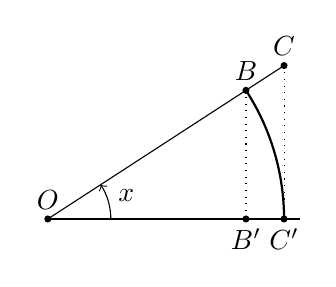
\begin{tikzpicture}
\pgfmathsetmacro{\r}{3};
\pgfmathsetmacro{\t}{33}
\coordinate (B) at ({\r*cos(\t)},{\r*sin(\t)});
\coordinate (Bp) at ({\r*cos(\t)},0);
\coordinate (C) at (\r,{(\r*sin(\t))/cos(\t)});
\coordinate (Cp) at (\r,0);
\draw[dotted] (B)--(Bp);
\draw[dotted] (C)--(Cp);
\draw (0,0)--(C);
\draw (0,0)--(\r+0.2,0);
\draw[thick] (\r,0) arc (0:\t:\r);
\fill (B) circle (0.45mm);
\fill (Bp) circle (0.45mm);
\fill (C) circle (0.45mm);
\fill (Cp) circle (0.45mm);
\draw (B) node[above]{$B$};
\draw (Bp) node[below]{$B'$};
\draw (C) node[above]{$C$};
\draw (Cp) node[below]{$C'$};
\fill (0,0) circle (0.45mm);
\draw (0,0) node[above]{$O$};
\pgfmathsetmacro{\b}{0.8};
\draw[->] (\b,0) arc (0:\t:\b);  
\draw ({\t/2}:{1.3*\b}) node{$x$};
\end{tikzpicture}\end{bmlimage}
\end{center}

Temos $|OC'|=|OB|=1$, $|B'B|=\sen x$, $|OB'|=\cos x$ e $|C'C|=\tan x$.
Observe que 
\[ 
\text{área do triângulo }OB'B\leq
\text{área do setor }OC'B\leq
\text{área do triângulo }OC'C.
\]
A área $\sigma$ do setor $OC'B$ se
calculada observando que por proporcionalidade:
$\frac{x}{2\pi}=\frac{\sigma}{\pi\cdot 1^2}$. Logo,
$\sigma=\frac{x}{2}$. Assim, reescrevendo as três desigualdades acima em termos
de $x$,
$$\tfrac12 \sen x\cos x\leq \tfrac12 x\leq \tfrac12 \tan x\,.$$
A primeira desigualdade implica $\sen x\cos x\leq x$, isto é,
$\frac{\sen x}{x}\leq \frac{1}{\cos x}$. A segunda implica 
$x\leq \tan x=\frac{\sen x}{\cos x}$,
isto é, $\cos x\leq \frac{\sen x}{x}$. Logo,
$$\cos x\leq \frac{\sen x}{x}\leq \frac{1}{\cos x}\,,\quad\forall 0<x<\pisobredois\,.
$$
Como $\lim_{x\to 0^+}\cos x=\lim_{x\to 0^+}\frac{1}{\cos x}=1$, O Teorema \ref{Teo:Sanduichefinito} implica
$\lim_{x\to 0^+}\frac{\sen x}{x}=1$.
Como $\frac{\sen x}{x}$ é par, temos também $\lim_{x\to
0^-}\frac{\sen x}{x}=1$. Portanto, provamos \eqref{eq_limsenxsurx}.

\begin{exo}\label{Exo:variantessinxsurx}
%\eqref{itexosinxx5}
Usando \eqref{eq_limsenxsurx}, calcule os limites 
\begin{multicols}{4}
\begin{enumerate}
\item\label{itexosinxx1} $\lim_{x\to 0}\tfrac{\tan x}{x}$
\item\label{itexosinxx2} $\lim_{x\to 0}\tfrac{\sen x}{\tan x}$
\item\label{itexosinxx3} $\lim_{x\to 0}\frac{\sen 2x}{\cos x}$
\item\label{itexosinxx4} $\lim_{x\to 0}\frac{\sen 2x}{x\cos x}$
\item\label{itexosinxx5} $\lim_{x\to 0}\tfrac{1-\cos x}{x^2}$
\item\label{itexosinxx6} $\lim_{x\to 0^+}\tfrac{\cos x}{x}$
\item\label{itexosinxx7} $\lim_{x\to 0^+}\tfrac{\sen (x^2)}{x}$
\end{enumerate}
\end{multicols}
\vspace{0.01cm}
\begin{sol} \eqref{itexosinxx1}
Como $\frac{\tan x}{x}=\frac{\sen x}{x}\frac{1}{\cos x}$,
temos $\lim_{x\to 0}\tfrac{\tan x}{x}=1$.
\eqref{itexosinxx2}
Como $\frac{\sen x}{\tan x}=\cos x$, temos $\lim_{x\to 0}\tfrac{\sen
x}{\tan x}=1$.
\eqref{itexosinxx3} Como ${\sen 2x}\to 0$ e ${\cos x}\to 1$, temos $\lim_{x\to 0}\frac{\sen 2x}{\cos x}=\frac{0}{1}=0$ (não é um limite do tipo ``$\frac00$'').
\eqref{itexosinxx4}
Como $\frac{\sen 2x}{x\cos x}=2\frac{\sen x}{x}$,
temos $\lim_{x\to 0}\frac{\sen 2x}{x\cos x}=2$.
\eqref{itexosinxx5} Como 
$$\frac{1-\cos x}{x^2}=\frac{1-\cos x}{x^2}\frac{1+\cos
x}{1+\cos x}=\frac{1-\cos^2x}{x^2}\cdot \frac{1}{1+\cos x}=\Bigl(\frac{\sen x}{x}\Bigr)^2\cdot \frac{1}{1+\cos x}\,,$$
temos 
$\lim_{x\to 0}\tfrac{1-\cos x}{x^2}=(1)^2\cdot \frac12=\frac12$.
\eqref{itexosinxx6} $+\infty$
\eqref{itexosinxx7}  $\lim_{x\to 0^+}\tfrac{\sen (x^2)}{x}=\lim_{x\to
0^+}x\cdot\tfrac{\sen(x^2)}{x^2}=0\cdot 1=0$.
\end{sol}
\end{exo}



\section{Limites laterais infinitos, assíntotas verticais}
\index{assíntota!vertical}
Vimos casos em que limites laterais são iguais, casos em que eles são 
diferentes, e casos em que eles nem existem. Vejamos agora casos em que
eles são \emph{infinitos}.

\begin{ex}
Considere primeiro $f(x)=\frac{1}{x}$. Já vimos que a $f$ não é
limitada, e à medida que $x>0$ tende a zero,
$\frac{1}{x}$ cresce e toma valores positivos arbitrariamente grandes.
Por outro lado se $x<0$ tende a zero, $\frac{1}{x}$ decresce e toma
valores negativos arbitrariamente grandes:
$$
\lim_{x\to 0^+}\frac{1}{x}=+\infty\,,\quad\quad \lim_{x\to
0^-}\frac{1}{x}=-\infty\,.
$$ 
De modo geral, qualquer $x^p$ com potência inteira negativa
$p=-q$, $q>0$:
$$
\lim_{x\to 0^+}\frac{1}{x^q}=+\infty\,,\quad\quad
\lim_{x\to 0^-}\frac{1}{x^q}=
\begin{cases}
+\infty&\text{ se $q$ é par\,,}\\
-\infty&\text{ se $q$ é ímpar\,.}
\end{cases}
$$
\end{ex}

\begin{exo}
Tente definir 
rigorosamente $\lim_{x\to a^+}f(x)=+\infty$, $\lim_{x\to a^+}f(x)=-\infty$.
\begin{sol}
``$\lim_{x\to a^+}f(x)=+\infty$'' significa que $f(x)$ ultrapassa
qualquer valor dado (arbitrariamente grande), desde que $x>a$ esteja
suficientemente perto de $a$. Isto é: para todo $M>0$ (arbitrariamente
grande), existe um $\delta>0$ tal que se $a<x\leq a+\delta$, então
$f(x)\geq M$.
Por outro lado, $\lim_{x\to a^+}f(x)=-\infty$ significa que 
para todo $M>0$ (arbitrariamente grande), 
existe um $\delta>0$ tal que se $a<x\leq a+\delta$, então $f(x)\leq
-M$.
\end{sol}
\end{exo}

\begin{defin}
 Se pelo menos um dos limites $\lim_{x\to a^+}f(x)$ ou $\lim_{x\to
a^-}f(x)$ é $\pm \infty$, diremos que a reta vertical de equação
$x=a$ é \grasA{assíntota vertical} da função $f$.
\end{defin}

\begin{ex} Como $\lim_{x\to 0^+}\log_ax=-\infty$ se $a>1$, $=+\infty$
se $0<a<1$, $x=0$ é assíntota vertical da função $\log_a$.
\end{ex}

\begin{ex}
A função tangente possui infinitas assíntotas verticais, 
de equações $x=\pisobredois+k\pi$, $k\in \bZ$, 
já que para todo $k\in \bZ$,
$$
\lim_{x\to (\pisobredois+k\pi)^-}\tan x=+\infty\,,\quad\quad
\lim_{x\to (\pisobredois+k\pi)^+}\tan x=-\infty\,.
$$
\end{ex}

\begin{exo}
Calcule os limites.
\begin{multicols}{3}
\begin{enumerate}
\item\label{itlimbasic9a} $\li{x}{2^+}\frac{x^2+5x+6}{x+2}$
\item\label{itlimbasic9b} $\li{x}{-2^+}\frac{x^2+5x+6}{x+2}$
\item\label{itlimbasic9c} $\li{x}{-2^\pm}\frac{x^2+5x-6}{x+2}$
\item\label{itlimbasic10} $\lim_{x\to 2^+}\frac{x-2}{(\sqrt{x^2-4})^2}$
\item\label{itlimbasic12} $\lim_{x\to -2^-}\frac{x-2}{(\sqrt{x^2-4})^2}$
\item\label{itlimbasic14} $\li{t}{0^+}\ln t-t$
\item\label{itlimbasic14b} $\li{t}{0^-}\ln t-t$
\item\label{itlimbasic15a} $\lim_{t\to 0^\pm}\frac{1}{\sen t}$
\item\label{itlimbasic15b} $\lim_{t\to 0^\pm}\frac{t}{\sen t}$
\item\label{itlimbasic15} $\lim_{t\to 0^+}\frac{\sen \frac1t}{t}$
\item\label{itlimbasic16} $\li{z}{0^\pm}9^{\frac{1}{z}}$
\item\label{itlimbasic18b} $\lim_{x\to 0^+}\ln \frac{1}{x}$
\item\label{itlimbasic19b} $\li{x}{0}\log(x^2)$
\item\label{itlimbasic13} $\lim_{x\to 0}\frac{e^x-1}{x}$
\end{enumerate}
\end{multicols}
\vspace{0.01cm}
\begin{sol}
\eqref{itlimbasic9a} $5$
\eqref{itlimbasic9b} $1$
\eqref{itlimbasic9c} $\mp \infty$
\eqref{itlimbasic10} Observe que enquanto $x^2-4>0$, $\frac{x-2}{(
\sqrt{x^2-4})^2}=\frac{1}{x+2}$. Logo, $\lim_{x\to
2^+}\frac{x-2}{(\sqrt{x^2-4})^2}=\frac14$, e
\eqref{itlimbasic12} $\lim_{x\to -2^-}\frac{x-2}{(\sqrt{x^2-4})^2}=
-\infty$
\eqref{itlimbasic14} $-\infty$
\eqref{itlimbasic14b} Não é definido.
\eqref{itlimbasic15a}   $\lim_{t\to 0^+}\frac{1}{\sen t}=+\infty$, 
$\lim_{t\to 0^-}\frac{1}{\sen t}=-\infty$
\eqref{itlimbasic15b}   $\lim_{t\to 0^\pm}\frac{t}{\sen t}=\lim_{t\to 
0^\pm}\frac{1}{\frac{\sen t}{t}}=1$.
\eqref{itlimbasic15} Não existe, porqué quando $t\to 0^+$, $\sen
\frac1t$ 
oscila entre $+1$ e $-1$, enquanto $\frac1t$ tende a $+\infty$:
\begin{center}
\begin{bmlimage}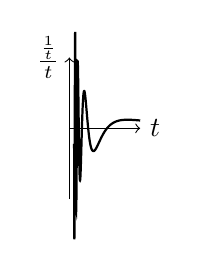
\begin{tikzpicture}[scale=0.3]
\draw[->] (0,0)--(3,0) node[right]{$t$};
\draw[->] (0,-3)--(0,3) node[left]{$\frac{\sen \frac1t}{t}$};
\pgfmathsetmacro{\e}{0.2};
\draw[thick, domain=\e:{3}, samples=1000] plot (\x,{(sin(5/\x r))/\x});
\end{tikzpicture}\end{bmlimage}
\end{center}
\eqref{itlimbasic16} $\li{z}{0^+}9^{\frac{1}{z}}=+\infty$, 
$\li{z}{0^-}9^{\frac{1}{z}}=0$.
\eqref{itlimbasic18b} $+\infty$
\eqref{itlimbasic19b} $-\infty$
\eqref{itlimbasic13} $1$ (veremos mais tarde como calcular esse
limite...) 
\end{sol}
\end{exo}

\begin{exo}
Na Teoria da Relatividade Restrita (ou Especial), cujo principal 
postulado é que a velocidade da luz é uma constante $c>0$ para
qualquer observador, 
é provado que a massa efetiva de uma partícula em movimento uniforme 
depende da sua velocidade. Se a massa no repouso é $m_0$, então a sua
massa efetiva quando a partícula tem uma
velocidade constante $v$ é dada por
$$m_v=\frac{m_0}{\sqrt{1-\frac{v^2}{c^2}}}\,.$$
Estude $m_v$ quando $v$ se aproxima da velocidade da luz.
\begin{sol}
A função $v\mapsto m_v$ tem domínio $[0,c)$, e a reta $v=c$ é 
assíntota vertical: 
\begin{center}
\begin{bmlimage}\begin{tikzpicture}
\draw[->] (0,0)--(4,0) node[right]{$v$};
\draw[->] (0,0)--(0,3) node[left]{$m_v$};
\pgfmathsetmacro{\c}{3.2};
\pgfmathsetmacro{\m}{1};
\fill (0,\m) circle (0.45mm);
\draw (0,\m) node[left]{$m_0$};
\draw[thick, domain=0:{\c-0.2}] plot (\x,{\m/(sqrt(1-(\x/\c)^2))});
\draw[dotted] (\c,0) node[below]{$c$}--(\c,3);
\draw (3.8,2.5) node[right]{$\displaystyle{\lim_{v\to c^-}m_v}=
+\infty$};
\end{tikzpicture}\end{bmlimage}
\end{center}
\end{sol}
\end{exo}

\begin{exo}
Considere $f(x)=\frac{x+1}{x-1}$. Estude os limites relevantes e 
ache as assíntotas (horizontais e verticais) de $f$. A partir dessas
informações, monte o gráfico de $f$.
\begin{sol}
Observe que $\lim_{x\to \pm\infty}f(x)=+1$, logo $y=1$ é assíntota 
horizontal. 
Por outro lado, $\lim_{x\to 1^+}f(x)=+\infty$ e $\lim_{x\to 1^-}f(x)
=-\infty$. Portanto, $x=1$ é assíntota vertical. 
Temos então: 1) o gráfico se aproxima da sua assintota horizontal em 
$-\infty$, e ele tende a $-\infty$ quando $x\to 1^-$,
2) o gráfico se aproxima da sua assintota horizontal em $+\infty$, e 
ele tende a $+\infty$ quando $x\to 1^+$.
Somente com essas informações, um esboço razoável pode ser montado: 
\begin{center}
\begin{bmlimage}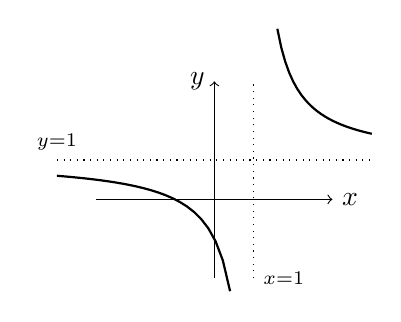
\begin{tikzpicture}[scale=0.5]
\draw[->] (-3,0)--(3,0) node[right]{$x$};
\draw[->] (0,-2)--(0,3) node[left]{$y$};
\pgfmathsetmacro{\e}{0.6};
%\pgfmathsetmacro{\m}{1};
%\fill (0,\m) circle (0.45mm);
%\draw (0,\m) node[left]{$m_0$};
\draw[thick, domain=-4:1-\e] plot (\x,{(\x+1)/(\x-1)});
\draw[thick, domain=1+\e:4] plot (\x,{(\x+1)/(\x-1)});
\draw[dotted] (1,-2) node[right]{$\scriptstyle{x=1}$}--(1,3);
\draw[dotted] (-4,1) node[above]{$\scriptstyle{y=1}$}--(4,1);
%\draw (3.8,2.5) node[right]{$\displaystyle{\lim_{v\to c^-}m_v}=+\infty$};
\end{tikzpicture}\end{bmlimage}
\end{center}
Observe que pode também escrever $\frac{x+1}{x-1}=\frac{2}{x-1}+1$, 
logo o gráfico pode ser obtido a partir de transformações elementares
do gráfico de $\frac1x$...
\end{sol}
\end{exo}

\begin{exo}
Dê o domínio e ache as assíntotas (horizontais e verticais), caso
existam, das funções 
\begin{multicols}{4}
\begin{enumerate}
\item\label{itexassint1} $2x+1$
\item\label{itexassint2} $\frac{1}{x+1}$
\item\label{itexassint3} $\frac{x^2-9}{x-3}$
\item\label{itexassint4} $\frac{2x-3}{x}$
\item\label{itexassint5} $\frac{1-x}{x+3}$
\item\label{itexassint6} $\frac{x}{x}$
\item\label{itexassint6b} $\log_5(2-x)$
\item\label{itexassint7} $x^3+\frac{1}{x}$
\item\label{itexassint8} $\frac{\sen x}{x}$
\item\label{itexassint9} $\frac{\cos x}{x}$
\item\label{itexassint10} $\frac{x^2+4x-21}{x^2-x+6}$
\item\label{itexassint11} $\ln(1-x^2)$
\item\label{itexassint12} $\frac{1}{2+x}+\ln(1-x^2)$
\item\label{itexassint13} $\frac{6-2x}{(1-x^2)(x-3)}$
\item\label{itexassint14} $\frac{1}{\ln(1-x^2)}$
\item\label{itexassint17} $\frac{\sqrt{x^2+1}}{x}$
\item\label{itexassint15b} $\frac{1}{\sqrt{1-x^2}}$
\item\label{itexassint18} $\frac{\ln(1+e^x)}{x}$
\end{enumerate}
\end{multicols}
\vspace{0.01cm}
\begin{sol}
\eqref{itexassint1} $D=\bR$, sem assíntotas.
\eqref{itexassint2} $D=\bR\setminus\{-1\}$. Horiz: $y=0$, Vertic: $x=-1$.
\eqref{itexassint3} $D=\bR\setminus\{3\}$. sem assíntotas.
\eqref{itexassint4} $D=\bR\setminus\{0\}$. Horiz: $y=2$, Vertic: $x=0$.
\eqref{itexassint5} $D=\bR\setminus\{-3\}$. Horiz: $y=-1$, Vertic: $x=-3$.
\eqref{itexassint6} $D=\bR\setminus\{0\}$. Horiz: $y=1$, Vertic: não tem.
\eqref{itexassint6b} $D=(-\infty,2)$. Horiz: não tem, Vertic: $x=2$.
\eqref{itexassint7} $D=\bR\setminus\{0\}$. Horiz: não tem, Vertic: $x=0$.
\eqref{itexassint8} $D=\bR\setminus\{0\}$. Horiz: $y=0$, Vertic: não tem.
\eqref{itexassint9} $D=\bR\setminus\{0\}$. Horiz: $y=0$, Vertic: $x=0$.
\eqref{itexassint10} $D=\bR$. Horiz: $y=1$, Vertic: não tem.
\eqref{itexassint11} Para garantir $1-x^2>0$, $D=(-1,1)$ Horiz: não 
tem (já que o domínio é $(-1,1)$...), Vertic: $x=-1$ (porqué
$\lim_{x\to -1^+}\ln (1-x^2)=-\infty$), $x=+1$ (porqué $\lim_{x\to
+1^-}\ln (1-x^2)=-\infty$).
\eqref{itexassint12} $D=(-1,1)$. Horiz: não tem, Vertic: $x=-1$, $x=+1$.
\eqref{itexassint13} $D=\bR\setminus\{\pm 1, 3\}$. Horiz: $y=0$, 
Vertic: $x=+1$, $x=-1$.
\eqref{itexassint14} $D=(-1,+1)\setminus\{ 0\}$. Horiz: não tem, 
Vertic: $x=0$.
\eqref{itexassint17} $D=\bR\setminus\{0\}$. Horiz: $y=+1$, $y=-1$, 
Vertic: $x=0$.
\eqref{itexassint15b} $D=(-1,1)$. Horiz: não tem, Vertic: $x=-1$, $x=+1$.
\eqref{itexassint18} $D=\bR\setminus\{0\}$. Horiz: $y=1$ (a direita), $y=0$ (a esquerda), 
Vertic: $x=0$.
\end{sol}
\end{exo}

\begin{exo}(Primeira prova, Turmas D, 15 de abril de 2011)
Defina \emph{assíntota horizontal/vertical} de uma função $f$, e 
ache as assíntotas das funções 
$$
\frac{|x-\pi|}{\pi+x}\,,\quad 
\frac{2+\sen x-3 x^2}{x^2-x+20}
\,,\quad \frac{\sqrt{x(x-1)}}{x-1}\,.$$
\end{exo}

\begin{exo}
Dê exemplos de funções $f$ que tenham $x=-1$ e
$x=3$ como assíntotas verticais, e $y=-1$ como assíntota
horizontal.
\begin{sol}
Por exemplo: $f(x)=\frac{1-x^2}{(x+1)(x-3)}$, ou $f(x)=\frac{1}{x+1}
+\frac{1}{x-3}-\frac{x^2}{x^2+1}$.
\end{sol}
\end{exo}

\section{Mudar de variável}
\index{mudança de variável}
O cálculo de um limite pode ser às vezes simplificado transformando
ele em outro limite, via uma \emph{mudança de variável}.

\begin{ex}
Suponha que se queira calcular o limite de $\frac{\sen 2x}{x}$ quando
$x\to 0$. Um jeito possível é de usar a identidade 
$\sen 2x=2\sen x\cos x$, escrevendo 
$$
\lim_{x\to 0}\frac{\sen 2x}{x}
=\lim_{x\to 0}2\frac{\sen x}{x}\cos x=2\cdot
1\cdot{1}=2\,.
$$
Um outro jeito de proceder é de introduzir a nova variável $y\pardef
2x$. Ao fazer essa mudança, é preciso reescrever o limite
$\lim_{x\to 0}\frac{\sen 2x}{x}$ somente usando a variável $y$. Como
$x\to 0$ implica $y\to 0$, e como $x=y/2$, 
$$
\lim_{x\to 0}\frac{\sen 2x}{x}
=\lim_{y\to 0}\frac{\sen y}{y/2}=2\lim_{y\to 0}\frac{\sen
y}{y}=2\cdot 1=2.$$
\end{ex}

\begin{ex} Considere o limite 
$\lim_{x\to 0}\frac{\cos^3x-1}{\cos x-1}$. Chamando $z\pardef \cos
x$, ao $x\to 0$ temos $z\to 1$. Logo, 
$$
\lim_{x\to 0}\frac{\cos^3x-1}{\cos x-1}=\lim_{z\to
1}\frac{z^3-1}{z-1}=3\quad\text{(ver Exemplo
\ref{Ex:primeironaotrivial}).}
$$
\end{ex}

Vejamos também como um limite lateral pode ser transformado em um
limite no infinito:

\begin{ex}
Considere os  limites laterais calculados no Exercício
\ref{Exo:Limiteselementares}: $\lim_{x\to 0^+}9^{\frac{1}{x}}$,
$\lim_{x\to 0^-}9^{\frac{1}{x}}$.
Chamemos $z\pardef \frac{1}{x}$. Se $x\to 0^+$, então $z\to
+\infty$. Logo,
$$\lim_{x\to 0^+}9^{\frac{1}{x}}
=\lim_{z\to\infty}9^z=+\infty\,.
$$
Por outro lado, se $x\to 0^-$, então $z\to -\infty$, e
$$\lim_{x\to 0^-}9^{\frac{1}{x}}
=\lim_{z\to-\infty}9^z=0\,.
$$
\end{ex}

\begin{exo}\label{Exo:mudvarlimites}
Calcule os limites fazendo uma mudança de variável.
\begin{multicols}{3}
\begin{enumerate}
\item\label{itmudvarlim1} $\lim_{x\to 1}\frac{\sen (x-1)}{3x-3}$
\item\label{itmudvarlim11} $\lim_{x\to 0}\frac{\sen (3x)}{\sen (5x)}$
\item\label{itmudvarlim2} $\lim_{x\to -1}\frac{\sen(x+1)}{1-x^2}$
\item\label{itmudvarlim3} $\lim_{x\to a}\frac{x^n-a^n}{x-a}$
\item\label{itmudvarlim31} $\lim_{x\to 4}\frac{x-4}{x-\sqrt{x}-2}$
\item\label{itmudvarlim4} $\lim_{x\to 0^{\pm}}\tanh \frac{1}{x}$
\item\label{itmudvarlim5} $\lim_{x\to 0^{\pm}}x\tanh \frac{1}{x}$
\end{enumerate}
\end{multicols}
\vspace{0.01cm}
\begin{sol}
\eqref{itmudvarlim1} Com $z\pardef x-1$, $\lim_{x\to 1}\frac{\sen
(x-1)}{3x-3}=\lim_{z\to 0}\frac{\sen
z}{3z}=\frac13$.
\eqref{itmudvarlim11} $\frac35$ (Escreve $\frac{\sen (3x)}{\sen (5x)}=\frac{\sen (3x)}{3x}\frac{1}{\frac{\sen (5x)}{5x}}\frac{3x}{5x}$.) 
\eqref{itmudvarlim2} Com $z\pardef x+1$, $\lim_{x\to
-1}\frac{\sen(x+1)}{1-x^2}=\lim_{z\to
0}\frac{\sen z}{z}\frac{1}{2-z}=\frac12$.
\eqref{itmudvarlim3} Com $h\pardef x-a$, 
$\lim_{x\to a}\frac{x^n-a^n}{x-a}=\lim_{h\to
0}\frac{(a+h)^n-a^n}{h}=na^{n-1}$.
\eqref{itmudvarlim31} Chamando $t\pardef \sqrt{x}$, 
$$\lim_{x\to 4}\frac{x-4}{x-\sqrt{x}-2}=\lim_{t\to 2}\frac{t^2-4}{t^2-t-2}=\lim_{t\to 2}\frac{(t-2)(t+2)}{(t-2)(t+1)}=\lim_{t\to 2}\frac{(t+2)}{(t+1)}=\tfrac43\,.$$
\eqref{itmudvarlim4} Com $z\pardef \frac{1}{x}$, temos (lembre o
item \eqref{itexliminfini22} do Exercício \ref{Exo:limitesinfini})
 $\lim_{x\to 0^+}\tanh \frac{1}{x}=\lim_{z\to +\infty}\tanh z=+1$,
$\lim_{x\to 0^-}\tanh \frac{1}{x}=\lim_{z\to -\infty}\tanh z=-1$.
\eqref{itmudvarlim5} Com a mesma mudança,
$\lim_{x\to 0^\pm}x\tanh \frac{1}{x}=\lim_{z\to \pm
\infty}\frac{1}{z}\tanh{z}=0\cdot (\pm 1)=0$.
\end{sol}
\end{exo}

\section{O limite $e=\lim_{x\to
\infty}\bigl(1+\tfrac1x\bigr)^x$}\label{Sec:Fundam_numero_e}

Mencionamos, no último capítulo, que uma das definições possíveis do
número $e=2,718...$ é via o limite de $(1+\tfrac1x)^x$
quando $x\to \infty$. De fato,
\begin{center}
\begin{tabular}{c|c|c|c|c}
$x=$&10&100&1000&10'000\\
\hline
$(1+\tfrac1x\bigr)^x=$&$2,59374...$&$2,70481...$&$2,
71692...$&$2.71814...$
\end{tabular}
\end{center}
Pode ser mostrado que o limite quando $x\to \infty$
existe, e tomamos o valor do limite como definição da base do logaritmo natural:
$$\boxed{e\pardef \lim_{x\to \infty}\bigl(1+\tfrac1x\bigr)^x\,.}$$

Essa caracterização de $e$ permite calcular vários limites importantes,
como por exemplo
$\lim_{h\to 0^+}\frac{\ln(1+h)}{h}$.
De fato, com a mudança de variável $z=\frac{1}{h}$, $h\to 0^+$ implica $z\to +\infty$:
\eq{\label{eq:usoimpliccontinlog}\lim_{h\to
0^+}\frac{\ln(1+h)}{h}=\lim_{z\to+\infty}\frac{\ln(1+\tfrac{1}{z})}{\frac1z}=
\lim_{z\to+\infty}\ln\bigl((1+\tfrac{1}{z})^z\bigr)
=\ln e=1\,.
}

Um outro limite que pode ser calculado é $\lim_{x\to 0^+}\frac{e^x-1}{x}$. Dessa
vez, chamando $z=e^x$, $x\to 0^+$ implica $z\to 1^+$:
$$
\lim_{x\to 0^+}\frac{e^x-1}{x}=\lim_{z\to 1^+}\frac{z-1}{\ln
z}=\lim_{z\to
1^+}\frac{1}{\frac{\ln z}{z-1}}$$
Mas agora se $h\pardef z-1$, então $z\to 1^+$ implica $h\to 0^+$, e 
por \eqref{eq:usoimpliccontinlog},
$$
\lim_{z\to 1^+}\frac{\ln z}{z-1}=\lim_{h\to 0^+}\frac{\ln (1+h)}{h}=1\,.
$$
Portanto, 
\eq{\label{Eq:derivexponenzero}
\lim_{x\to 0^+}\frac{e^x-1}{x}=1\,.}
Observe que o limite lateral a esquerda se obtém facilmente: chamando $y\pardef -x$,
\begin{align*}
\lim_{x\to 0^-}\frac{e^x-1}{x}
=\lim_{y\to 0^+}\frac{e^{-y}-1}{-y}&=\lim_{y\to 0^+}\frac{e^{y}-1}{y}e^{-y}\\
&=\Bigl(\lim_{y\to 0^+}\frac{e^{y}-1}{y}\Bigr)\bigl(\lim_{y\to 0^+}e^{-y}\bigr)=1\cdot 1=1\,.
\end{align*}


\begin{exo}
Mostre que  para todo $a>0$,
\eq{\label{eq:derivlnenun}\lim_{h\to
0}\frac{\log_a(1+h)}{h}=\frac{1}{\ln a}\,,\quad\quad \lim_{x\to
0}\frac{a^x-1}{x}=\ln a\,.}
\begin{sol}
Pela fórmula \eqref{eq:mudancabaselog} de mudança de base para o
logaritmo, $\log_a(1+h)=\frac{\ln(1+h)}{\ln a}$. Logo, por
\eqref{eq:derivlnenun},
$$\lim_{h\to 0}\frac{\log_a(1+h)}{h}=\frac{1}{\ln a}\lim_{h\to
0}\frac{\ln(1+h)}{h}=\frac{1}{\ln a}\,.$$
Por outro lado, chamando $z\pardef a^x$, $x\to 0$ implica $z\to 1$.
Mas $x=\log_az$, logo
$$
\lim_{x\to
0}\frac{a^x-1}{x}=\lim_{z\to 1}\frac{z-1}{\log_a
z}=\frac{1}{\lim_{z\to 1}\frac{\log_az}{z-1}}\,.
$$
Definindo $h\pardef z-1$ obtemos $\lim_{z\to
1}\frac{\log_az}{z-1}=\lim_{h\to 0}\frac{\log_a(1+h)}{h}=\frac{1}{\ln
a}$, o que prova a identidade desejada.
\end{sol}
\end{exo}

\section{O limite 
$\lim_{x\to\infty}\frac{a^x}{x}$}\label{sec_Lim_parenteseAldo}
Nesta seção
%~\footnote{Essa seção foi escrita após a proposta
%do Prof.\ Aldo Procacci.} 
veremos como calcular alguns limites que envolvem
exponenciais e logaritmos, do tipo 
\[ 
\lim_{x\to\infty}\frac{e^x}{x}\,, \quad
\lim_{x\to\infty}\frac{(\ln x)^3}{x}\,, \dots\quad
\]
Esses limites costumam ser estudados usando a regra de
Bernoulli-l'Hôpital, que será vista no
Capítulo~\ref{Cap:Derivacao}. 
Será suficiente considerar um caso.
\begin{ex}
Mostraremos aqui que
\begin{equation}\label{eq_Lim_ideiaaldo} 
\boxed{
\lim_{x\to\infty}\frac{a^x}{x}=
\begin{cases}
+\infty&\text{ se }a>1\,,\\
0&\text{ se }0<a\leq 1\,.
\end{cases}
}
\end{equation}
Quando $a=1$, o limite é simplesmente
$\lim_{x\to\infty}\frac{a^0}{x}=
\lim_{x\to\infty}\frac{1}{x}=0$.
Quando $0<a<1$, temos $\lim_{x\to\infty}a^x=0$ (lembre
de~\eqref{eq_Lim_expinf_c}), o que implica
$\lim_{x\to\infty}\frac{a^x}{x}=
\lim_{x\to\infty}a^x\cdot\frac{1}{x}=0\cdot 0=0$.
Portanto, falta tratar o caso $a>1$.
Observe que nesse caso, podemos escrever $a=1+\beta$, com
$\beta>0$. 
\[ 
\frac{a^x}{x}=\frac{(1+\beta)^x}{x}\,.
\]
Suponhamos agora que $x>0$ seja grande. 
Como $x\geq \lfloor x \rfloor$, temos $(1+\beta)^x\geq
(1+\beta)^{\lfloor x \rfloor}$.
Agora, como $\lfloor x\rfloor$ é \emph{inteiro}. 
Assim podemos usar a fórmula do binômio de
Newton~\footnote{$(A+B)^n=\sum_{k=0}^n\binom{n}{k}A^kB^{n-k}$. Aqui 
usamos essa fórmula com $A=1$, $B=\beta$.}: 
\begin{align*}
(1+\beta)^{\lfloor x\rfloor}&=1+\beta
{\lfloor x\rfloor}+\beta^2\frac{{\lfloor x\rfloor}({\lfloor x\rfloor}-1)}{2}+\dots+\frac{{\lfloor x\rfloor}({\lfloor x\rfloor}-1)}{2}\beta^{\lfloor x\rfloor}\\
&\geq \beta^2\frac{{\lfloor x\rfloor}({\lfloor x\rfloor}-1)}{2}\,.
\end{align*}
Nesta última desigualdade observamos que 
todos os termos da soma são positivos, 
e mantivemos somente o termo de ordem $2$.
Portanto,
$\frac{a^x}{x} \geq \beta^2\frac{{\lfloor x\rfloor}^2-{\lfloor x\rfloor}}{2{x}}$.
Mas, como
\[ 
\lim_{x\to \infty}\frac{{\lfloor x\rfloor}^2-{\lfloor
x\rfloor}}{2{ x}}=+\infty\,, \]
provamos o resultado desejado:
$\lim_{x\to\infty}\frac{a^x}{x}=+\infty$.
\end{ex}

\begin{ex}
Podemos usar o último exemplo para mostrar que 
se $a>1$, então para todo inteiro $p>0$,
\begin{equation}\label{eq_Limlimlimlog} 
\boxed{
\lim_{x\to\infty}\frac{a^x}{x^p}=+\infty\,.
}
\end{equation}
De fato, podemos sempre escrever
$\frac{a^x}{x^p}=(\frac{b^x}{x})^p$, em que $b=a^{1/p}$. Como
$a>1$, vale $b>1$ também. Logo, por~\eqref{eq_Lim_ideiaaldo},
\[ 
\lim_{x\to\infty}\frac{a^x}{x^p}=
\lim_{x\to\infty}\bigl(\frac{b^x}{x}\bigr)^p=
\Bigl(\lim_{x\to\infty}\frac{b^x}{x}\Bigr)^p=+\infty\,.
\]
\end{ex}
A partir dos exemplos anteriores podemos calcular outros
limites: para todo $a>1$ e todo inteiro $p>0$,
\[ 
\boxed{
\lim_{x\to\infty}\frac{(\log_a x)^p}{x}=0
}
\]
De fato, com a mudança $y=\log_a x$, $x\to\infty$ implica
$y\to \infty$, logo por~\eqref{eq_Limlimlimlog}
\[ 
\lim_{x\to\infty}\frac{(\log_a x)^p}{x}=
\lim_{y\to\infty}\frac{y^p}{a^y}=
\lim_{y\to\infty}\frac{1}{\frac{a^y}{y^p}}=0\,.
\]
\begin{exo}
Calcule os limites abaixo.  
\begin{multicols}{3}
\begin{enumerate}
\item\label{it_exsuplAldo_1}
$\lim_{x\to\infty}\frac{e^{x}}{x^3}$
\item\label{it_exsuplAldo_2}
$\lim_{x\to\infty}\frac{0.5^x(\tfrac{18}{8})^x}{x^{16}}$
\item\label{it_exsuplAldo_3}
$\lim_{x\to\infty}\frac{e^{-2x}}{x}$
\item\label{it_exsuplAldo_4}
$\lim_{x\to\infty}\frac{e^{5x}}{x^{-2}}$
\item\label{it_exsuplAldo_5}
$\lim_{x\to\infty}\frac{(\log_3x)^{7}}{4x}$
\item\label{it_exsuplAldo_6}
$\lim_{x\to\infty}\frac{e^{2x}+3x^5}{(e^x+1)^2+2x^3}$
\end{enumerate}
\end{multicols}
\vspace{0.1mm}
\begin{sol}
\eqref{it_exsuplAldo_1} $\infty$
\eqref{it_exsuplAldo_2} $\infty$
\eqref{it_exsuplAldo_3} $0$
\eqref{it_exsuplAldo_4} $\infty$
\eqref{it_exsuplAldo_5} $0$
\eqref{it_exsuplAldo_6} $1$
\end{sol}
\end{exo}

\section{Exercícios de revisão}

\begin{exo}
Considere a função 
$$f(x)=
\begin{cases}
2x+2&\text{ se }x<0\,,\\
x^2-2&\text{ se }0\leq x<2\,,\\
2&\text{ se }x\geq 2\,.\\
\end{cases}
$$
Calcule os limites 
$\lim_{x\to 0^-}f(x)$,
$\lim_{x\to 0^+}f(x)$, $\lim_{x\to 0}f(x)$, $\lim_{x\to 2^-}f(x)$, $\lim_{x\to 2^+}f(x)$, 
$\lim_{x\to 2}f(x)$. Em seguida, interprete esses limites no gráfico de $f$.
\begin{sol}
$\lim_{x\to 0^-}f(x)=\lim_{x\to 0^-}(2x+2)=2$,
$\lim_{x\to 0^+}f(x)=\lim_{x\to 0^+}(x^2-2)=-2$,
Já que esses dois limites laterais são diferentes, $\lim_{x\to 0}f(x)$ não
existe.
$\lim_{x\to 2^-}f(x)=\lim_{x\to 2^-}(x^2-2)=2$.
$\lim_{x\to 2^+}f(x)=\lim_{x\to 2^+}2=2$. Como
$\lim_{x\to 2^-}f(x)=\lim_{x\to 2^+}f(x)$, $\lim_{x\to 2}f(x)$ existe e vale
$2$.
\begin{center}
\begin{bmlimage}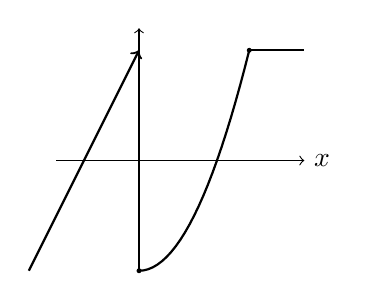
\begin{tikzpicture}[scale=0.7]
\draw[->] (-1.5,0)--(3,0)node[right]{$x$};
\draw[->] (0,-2)--(0,2.4);
\draw[->, thick] (-2,-2)--(0,2);
\fill (0,-2) circle (0.45mm);
\draw[thick, domain=0:2] plot (\x,{\x^2-2});
\fill (2,2) circle (0.45mm);
\draw[thick] (2,2)--(3,2);
\end{tikzpicture}\end{bmlimage}
\end{center}
\end{sol}
\end{exo}

\begin{exo}
Considere um ponto $Q$ na parábola $y=x^2$.
Seja $M$ o ponto meio do segmento $OQ$ ($O$ é a origem) e seja
$r$ a reta perpendicular ao segmento $OQ$, passando por $M$. Seja $R$
a interseção de $r$ com o eixo $y$. Estude o que acontece com $R$ quando
$Q$ varia. O que acontece com $R$ no limite $Q\to O$?
\begin{sol}
O ponto $Q$ é da forma $Q=(\lambda,\lambda^2)$, e $Q\to O$
corresponde a $\lambda\to 0$.
Temos $M=(\frac{\lambda}{2},\frac{\lambda^2}{2})$. 
É fácil ver que a equação da reta $r$ é 
$y=-\frac{1}{\lambda}x+\frac{\lambda^2}{2}+\frac12$. Logo,
$R=(0,\frac{\lambda^2}{2}+\frac12)$. Quando $Q$ se aproxima da origem,
isto é, quando $\lambda$ se aproxima de $0$, $\lambda^2$ decresce,
o que significa que $R$ \emph{desce}. Quando $\lambda\to 0$, $R\to
(0,\frac12)$. (Pode parecer contra-intuitivo, já que o segmento $OQ$ tende a
ficar sempre mais horizontal, logo o segmento $MR$ fica mais vertical, à medida
que $Q\to O$.)
\end{sol}
\end{exo}

\begin{exo}\label{Exo:DecomporCircemTriang}
Considere um círculo $C$ de raio $r>0$. Considere a divisão de $C$ em $n$
setores de aberturas iguais. 
Aproxime a área de cada setor pela área de um triângulo,
escreva a área $A_n$ do polígono definido pela união dos $n$ triângulos, e
calcule $\lim_{n\to \infty}A_n$.
\begin{sol}\mbox{}
\begin{center}
\begin{bmlimage}\begin{tikzpicture}
\pgfmathsetmacro{\r}{2};
\pgfmathsetmacro{\n}{10};
\pgfmathsetmacro{\incrang}{2*3.14152/\n};
\draw (0,0) circle (\r);
\foreach \k in {0,...,\n} {
\coordinate (Pk) at ({\r*cos(\k*\incrang r)},{\r*sin(\k*\incrang r)});
\coordinate (Pkm) at ({\r*cos((\k-1)*\incrang r)},{\r*sin((\k-1)*\incrang
r)});
\fill[color=gray!10] (0,0)--(Pk)--(Pkm)--cycle;
\draw (0,0)--(Pk)--(Pkm);
}
\coordinate (Pk) at ({\r*cos(\incrang r)},{\r*sin(\incrang r)});
\coordinate (Pkm) at ({\r*cos(0 r)},{\r*sin(0 r)});
\coordinate (M) at ($(Pk)!(0,0)!(Pkm)$);
\fill[color=gray!30] (0,0)--(Pk)--(Pkm)--cycle;
\draw[thick] (0,0)--(Pk)--(Pkm)--cycle;
\draw[thick] (0,0)--(M);
%\draw (M) node[above right]{$M$};
\end{tikzpicture}\end{bmlimage}
\end{center}
Como um setor tem abertura $\alpha_n=\frac{2\pi}{n}$, 
a área de cada triângulo se calcula facilmente:
$$2\times \frac12
\times(r\cos\tfrac{\alpha_n}{2})\times
(r\sen\tfrac{\alpha_n}{2})=\frac{r^2}{2}\sen
{\alpha_n}=\frac{r^2}{2}\sen \tfrac{2\pi}{n}\,.$$
Logo, a área do polígono é dada por $A_n=n\times \frac{r^2}{2}\sen
\frac{2\pi}{n}$. No limite $n\to \infty$ obtemos
$$
\lim_{n\to \infty}A_n=r^2\lim_{n\to \infty}\frac{n}{2}\sen \frac{2\pi}{n}
=\pi r^2\lim_{n\to \infty}\frac{1}{\frac{2\pi}{n}}\sen \tfrac{2\pi}{n}
=\pi r^2\lim_{t\to 0^+}\frac{\sen t}{t}=\pi r^2\,.
$$
\end{sol}
\end{exo}

\begin{exo}
Calcule o limite, se existir.
\begin{multicols}{3}
\begin{enumerate}
\item\label{itrevisaolimites1} $\lim_{x\to 2}\frac{x^4-16}{x-2}$
\item\label{itrevisaolimites11} $\lim_{x\to \frac13}\frac{3x^2-x}{3x-1}$
\item\label{itrevisaolimites2} $\lim_{x\to 3}\frac{x^2+4x-21}{x^2-x-6}$
\item\label{itrevisaolimites3} $\lim_{x\to 3}\frac{x^2+4x-21}{x^2-x+6}$
\item\label{itrevisaolimites31} $\lim_{x\to \infty}\frac{x^2+4x-21}{x^2-x+6}$
\item\label{itrevisaolimites4} $\lim_{x\to\infty}\frac{x^3+1}{x^3+x^2-2x^3}$
\item\label{itrevisaolimites5} $\lim_{x\to -1}\frac{\sen(x+1)}{1-x^2}$
\item\label{itrevisaolimites6} $\lim_{x\to 0}\frac{\sen x}{(\cos x)^2}$
\item\label{itrevisaolimites7} $\lim_{x\to 0^+}\log_9(\sen(x))$
\item\label{itrevisaolimites8} $\lim_{x\to 0^+}\log_9(\cos(x))$
\item\label{itrevisaolimites9} $\lim_{x\to 0}\frac{1-\cos x}{x}$
\item\label{itrevisaolimites10} $\lim_{x\to 0}(\frac1x-\frac{1}{e^x-1})$ 
\item\label{itrevisaolimites12} $\scriptstyle{
\li{x}{\pm \infty}\sqrt{x^2-\pi
x}-\sqrt{x^2-1}}$
\item\label{itrevisaolimites13}
$\li{x}{+\infty}\sen(\frac{\pi}{2}+\frac{1}{1+x^2})$
\item\label{itrevisaolimites14} $\li{x}{+\infty}\frac{x^2+3}{5+x^3}$
\item\label{itrevisaolimites15} $\li{x}{+\infty}\frac{1-x^7}{10x^7+1}$
\item\label{itrevisaolimites16} $\lim_{h\to 0}\frac{\sqrt{3+3h}-\sqrt{3}}{h}$
\item\label{itrevisaolimites161} $\lim_{h\to 1}\frac{\sqrt[3]{h}-1}{\sqrt{h}-1}$
\item\label{itrevisaolimites17} $\lim_{x\to
-\infty}\frac{5x^2+8x-3}{7x^3-4x-17}$
\item\label{itrevisaolimites20} $\lim_{x\to 0}\frac{x\sen x}{2-2\cos x}$
\item\label{itrevisaolimites21} $\lim_{x\to
0}\frac{1-\sqrt{1-4x^2}}{2 x}$
\end{enumerate}
\end{multicols}
\vspace{0.01cm}
\begin{sol}
\eqref{itrevisaolimites1} $32$
\eqref{itrevisaolimites11} $\frac13$
\eqref{itrevisaolimites2} $2$
\eqref{itrevisaolimites3} $0$
\eqref{itrevisaolimites31} $1$
\eqref{itrevisaolimites4} $-1$
\eqref{itrevisaolimites5} Com a mudança $y=x+1$, $\frac12$
\eqref{itrevisaolimites6} $0$
\eqref{itrevisaolimites7} $-\infty$
\eqref{itrevisaolimites8} $0$
\eqref{itrevisaolimites9} $0$
\eqref{itrevisaolimites10} $\tfrac12$ (Pois é, esse limite é
um pouco mais difícil. Calcularemos ele no
Capítulo~\ref{Cap:Derivacao} usando a regra de
Bernoulli-l'Hôpital.)
\eqref{itrevisaolimites12} $\mp \pisobredois$
\eqref{itrevisaolimites13} Como $\sen$ é contínua em $\pisobredois$,
$\li{x}{+\infty}\sen(\frac{\pi}{2}+\frac{1}{1+x^2})=\sen(\frac{
\pi}{2}+\li{x}{+\infty}\frac{1}{1+x^2})=\sen \pisobredois =1$.
\eqref{itrevisaolimites14} $0$
\eqref{itrevisaolimites15} $-\frac{1}{10}$
\eqref{itrevisaolimites16} $\frac{\sqrt{3}}{2}$
\eqref{itrevisaolimites161} $\frac{2}{3}$
\eqref{itrevisaolimites17} $0$
\eqref{itrevisaolimites20} $1$ 
\eqref{itrevisaolimites21} $1$ 
\end{sol}
\end{exo}

\begin{exo} Prove o Teorema \ref{Teo:Sanduicheinfinito}.
\begin{sol}
Seja $\epsilon>0$ e $N$ grande o suficiente, tal que $|g(x)-\ell|\leq \epsilon$ e $|h(x)-\ell|\leq \epsilon$ para todo $x\geq N$.
Para esses $x$, podemos escrever $f(x)-\ell \leq h(x)-\ell\leq |h(x)-\ell|\leq \epsilon$, e $f(x)-\ell\geq g(x)-\ell\geq -|g(x)-\ell|\geq -\epsilon$. Logo, $|f(x)-\ell|\leq \epsilon$.
\end{sol}
\end{exo}

\begin{exo}\label{Exo:LimitescomDicas}
Calcule os limites 
%\begin{multicols}{2}
\begin{enumerate}
\item\label{itlimdificeis0} $\lim_{x\to 0}\frac{\sqrt{1-\cos x}}{|x|}$ (Dica:
$1-\cos^2 x=\dots$) 
\item\label{itlimdificeis1} $\lim_{h\to 0}\frac{\sen (a+h)-\sen a}{h}$ (Dica:
$\sen (a+b)=\dots$)
\item\label{itlimdificeis2} $\lim_{x\to \alpha}\frac{x^3-\alpha^3}{\sen
(\tfrac{\pi}{\alpha}x)}$ (Dica: $\lim_{x\to
\alpha}\frac{x^3-\alpha^3}{x-\alpha}=\dots$)
\item\label{itlimdificeis3} Para $a,b>0$, $\lim_{x\to \pisobretres}\frac{1-2\cos
x}{\sen(\pi-3x)}$ (Dica: $\pi-3x=3t$, $\cos (a+b)=\dots$)
\item\label{itlimdificeis34} $\lim_{x\to\infty}\frac1x\ln(a^x+b^x)$ (Dica:
distinguir $a\geq b$, $a<b$)
\item\label{itlimdificeis37}
Para $n\in \bN$, $x_0\in \bR$, 
$\lim_{h\to 0}\frac{(x+h)^n-x^n}{h}$ 
(Dica: use uma mudança de variável $z=x+h$ e faça uma
divisão, ou então
use a fórmula do binômio de Newton para expandir $(x_0+h)^n$.)
\end{enumerate}
%\end{multicols}
\begin{sol}
\eqref{itlimdificeis0} Como $\sqrt{1-\cos^2x}=\sqrt{\sen^2x}=|\sen x|$ e
$x\mapsto |x|$ é contínua,
$$\lim_{x\to 0}\frac{\sqrt{1-\cos x}}{|x|}=\lim_{x\to
0}\frac{1}{\sqrt{1+\cos x}}\frac{|\sen x|}{|x|}
=\Bigl(\lim_{x\to 0}\frac{1}{\sqrt{1+\cos x}}\Bigr)
\cdot \Bigl|
\lim_{x\to 0}\frac{\sen x}{x}\Bigr|=\frac{1}{\sqrt{2}}\,.
$$
\eqref{itlimdificeis1} Como $\sen (a+h)=\sen a\cos h+\sen h\cos a$, temos
$$
\lim_{h\to 0}\frac{\sen (a+h)-\sen a}{h}=\sen a \Bigl(\lim_{h\to 0}\frac{\cos
h-1}{x}\Bigr)+\cos a\Bigl(\lim_{h\to 0}\frac{\sen h}{h}\Bigr)=\cos a\,.
$$
\eqref{itlimdificeis2} Escrevendo 
$$
\frac{x^3-\alpha^3}{\sen (\tfrac{\pi}{\alpha}x)}=
\frac{x^3-\alpha^3}{x-\alpha}\frac{1}{\frac{\sen
(\tfrac{\pi}{\alpha}x)}{x-\alpha}}\,.
$$
Já calculamos $\lim_{x\to \alpha}\frac{x^3-\alpha^3}{x-\alpha}= 3\alpha^2$, e 
chamando $y\pardef \tfrac{\pi}{\alpha}x$ seguido por $y'\pardef y-\pi$,
$$\lim_{x\to \alpha}\frac{\sen(\tfrac{\pi}{\alpha}x)}{x-\alpha}
=\lim_{y\to \pi}\frac{\sen(y)}{\frac{\alpha}{\pi}(y-\pi)}
=\frac{\pi}{\alpha}\lim_{y'\to 0}\frac{\sen(y'+\pi)}{y'}
=-\frac{\pi}{\alpha}\lim_{y'\to 0}\frac{\sen(y')}{y'}=-\frac{\pi}{\alpha}\,.$$
Logo,
$$
\lim_{x\to \alpha}\frac{x^3-\alpha^3}{\sen
(\tfrac{\pi}{\alpha}x)}=(3\alpha^2)/ (-\frac{\pi}{\alpha})=-3\alpha^3/ \pi\,.
$$
\eqref{itlimdificeis3} Comecemos definindo $t$ tal que $\pi-3x=3t$, isto é:
$t\pardef \pisobretres-x$:
$$\lim_{x\to \pisobretres}\frac{1-2\cos
x}{\sen(\pi-3x)}=\lim_{t\to 0}\frac{1-2\cos (\pisobretres-t)}{\sen (3t)}\,.$$
Mas $\cos (\pisobretres-t)=\cos \pisobretres\cos t+\sen \pisobretres\sen
t=\frac12\cos t+\frac{\sqrt{3}}{2}\sen t$,
\begin{align*}
\lim_{t\to 0}\frac{1-2\cos (\pisobretres-t)}{\sen (3t)}&=
\lim_{t\to 0}\frac{1-\cos t}{\sen (3t)}-\sqrt{3}\lim_{t\to 0}\frac{\sen
(t)}{\sen (3t)}\\
&=\lim_{t\to 0}\frac{1-\cos t}{t}\frac{1}{
3\frac{\sen (3t)}{3t}}-
\sqrt{3}\lim_{t\to
0}\frac{\sen (t)}{t}\frac{1}{3\frac{\sen
(3t)}{3t}}=0-\sqrt{3}\frac{1}{3}=-\frac{1}{\sqrt{3}}\,.
\end{align*}
\eqref{itlimdificeis34}
Se $a\geq b$, é melhor escrever $a^x+b^x=a^x(1+(b/a)^x)$, logo
\[ 
\lim_{x\to\infty}\frac{1}{x}\ln(a^x+b^x)
=\ln a+ 
\lim_{x\to\infty}\frac{\ln(1+(b/a)^x)}{x}
=\ln a\,.
\]
O caso $a<b$ se trata da mesma maneira. Obtemos:
\[ 
\lim_{x\to\infty}\frac{1}{x}\ln(a^x+b^x)
=
\begin{cases}
\ln a&\text{ se }a\geq b\,,\\
\ln b&\text{ se }a< b\,.\\
\end{cases}
\]
\eqref{itlimdificeis37}
O caso $n=1$ é trivial: $(x_0+h)^1=x_0+h$. Quando $n=2$, 
$(x_0+h)^2=x_0^2+2x_0h+h^2$, logo (veja o Exemplo
\ref{Ex:derivxissdoisemum})
$$
\lim_{h\to 0}\frac{(x_0+h)^2-x_0^2}{h}=
\lim_{h\to 0}(2x_0+h)=2x_0\,.
$$
Para $n=3,4,\dots$, usaremos a fórmula do binômio de
Newton:
$$(x_0+h)^n=x_0^n+\binom{n}{1}x_0^{n-1}h+\binom{n}{2}x_0^{n-2}
h^2+\dots+\binom{n}{k}x_0^{n-k} h^k+\dots+h^n\,,
$$
onde $\binom{n}{k}=\frac{n!}{(n-k)!k!}$. Portanto,
$$
\frac{(x_0+h)^n-x_0^n}{h}=\binom{n}{1}x_0^{n-1}+\binom{n}{2}x_0^{n-2}
h+\dots+\binom{n}{k}x_0^{n-k} h^{k-1}+\dots+h^{n-1}\,.
$$
Observe que cada termo dessa soma, a partir do segundo, contém
uma potência de $h$. Logo, quando $h\to 0$, só sobra 
o primeiro termo: $\binom{n}{1}x_0^{n-1}=nx_0^{n-1}$. Logo,
\[
\lim_{h\to 0}\frac{(x_0+h)^n-x_0^n}{h}=nx_0^{n-1}\,.
\]
Esse limite será usado para \emph{derivar} polinômios, no próximo capítulo.
\end{sol}
\end{exo}



